\newcommand{\foo}{\hspace{-2.3pt}$\bullet$ \hspace{5pt}}

\begin{frame}
  \begin{center}
    {\color{Maroon}\Huge Introduction}
  \end{center}
\end{frame}

%% put section outline here
\begin{frame}{Introduction}{Outline}
  \begin{enumerate}
  \item The shift in speech based user interfaces
  \item Building applications on the information rich speech signal
  \item The Speech Recognition Case Study
    \begin{itemize}
    \item From rule-based systems to data-driven system
    \item Impact of speech recognition technologies across languages and domains
    \item What is under the hood for speech recognition technologies?
    \item Building various ASR module and the impact of data
    \end{itemize}
  \item Building ASR Systems in New Languages
    \begin{itemize}
    \item Building from ASR systems from scratch
    \item Is there room for sharing data from other languages?
    \end{itemize}
  \item Building ASR Systems in New Domain
    \begin{itemize}
    \item Adaptation of an existing ASR system
    \end{itemize}
  \end{enumerate}
\end{frame}

\begin{frame}{Speech based user interfaces}{}
\begin{columns}[T]
    \column{2.5in}
     \alert{Star Trek's Universal Translator} [Wikipedia] -  \dots used in the late 22nd century on 
     Earth for the \alert{instant translation of well-known Earth languages}. Gradually, with 
     the removal of language barriers, Earth's disparate cultures came to terms of 
     universal peace. Translations of \alert{previously unknown languages}, such as those of 
     aliens, required more difficulties to be overcome. 
     \column{2in}
     \vspace{1cm}
     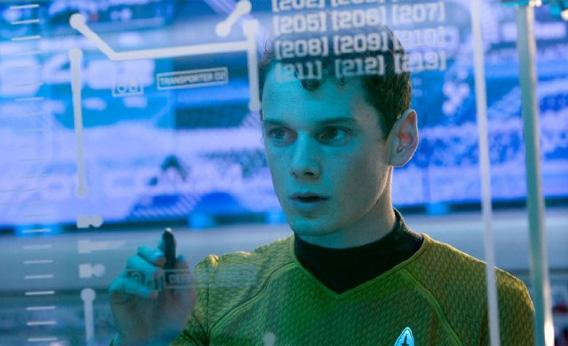
\includegraphics[height=30mm]{figures/startrek_comp}
  \end{columns}
\end{frame}

\begin{frame}{Speech based user interfaces}{}
\begin{columns}[T]
    \column{3in}
     \alert{Star Trek's The Next Generation Technical Manual} [Wikipedia] -  \dots the Universal Translator 
     is an "extremely sophisticated computer program" which functions by \alert{analyzing the patterns} of an unknown 
     foreign language, starting from \alert{a speech sample of two or more speakers in conversation}. The more extensive 
     the conversational sample, the more accurate and reliable is the "translation matrix," enabling instantaneous 
     conversion of verbal utterances or written text between the alien language and Federation Standard.
     \column{1in}
     \vspace{1.2cm}
     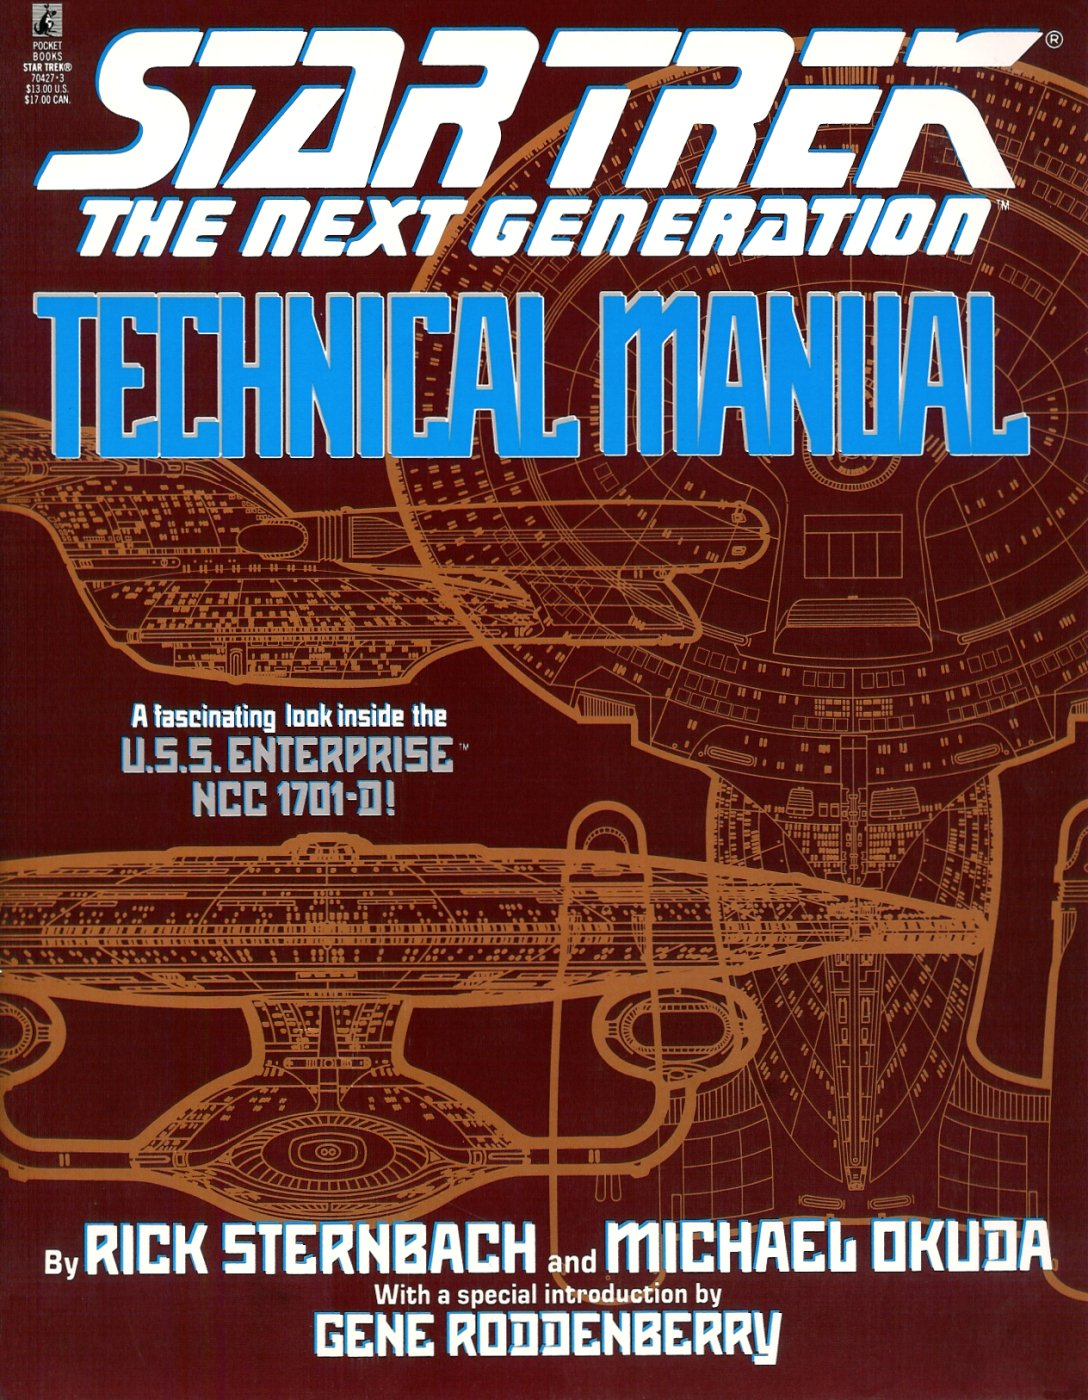
\includegraphics[height=40mm]{figures/startrek_manual}
  \end{columns}
\end{frame}

% Various applications that can be built on the speech signal
\begin{frame}{Building applications on the speech signal}
   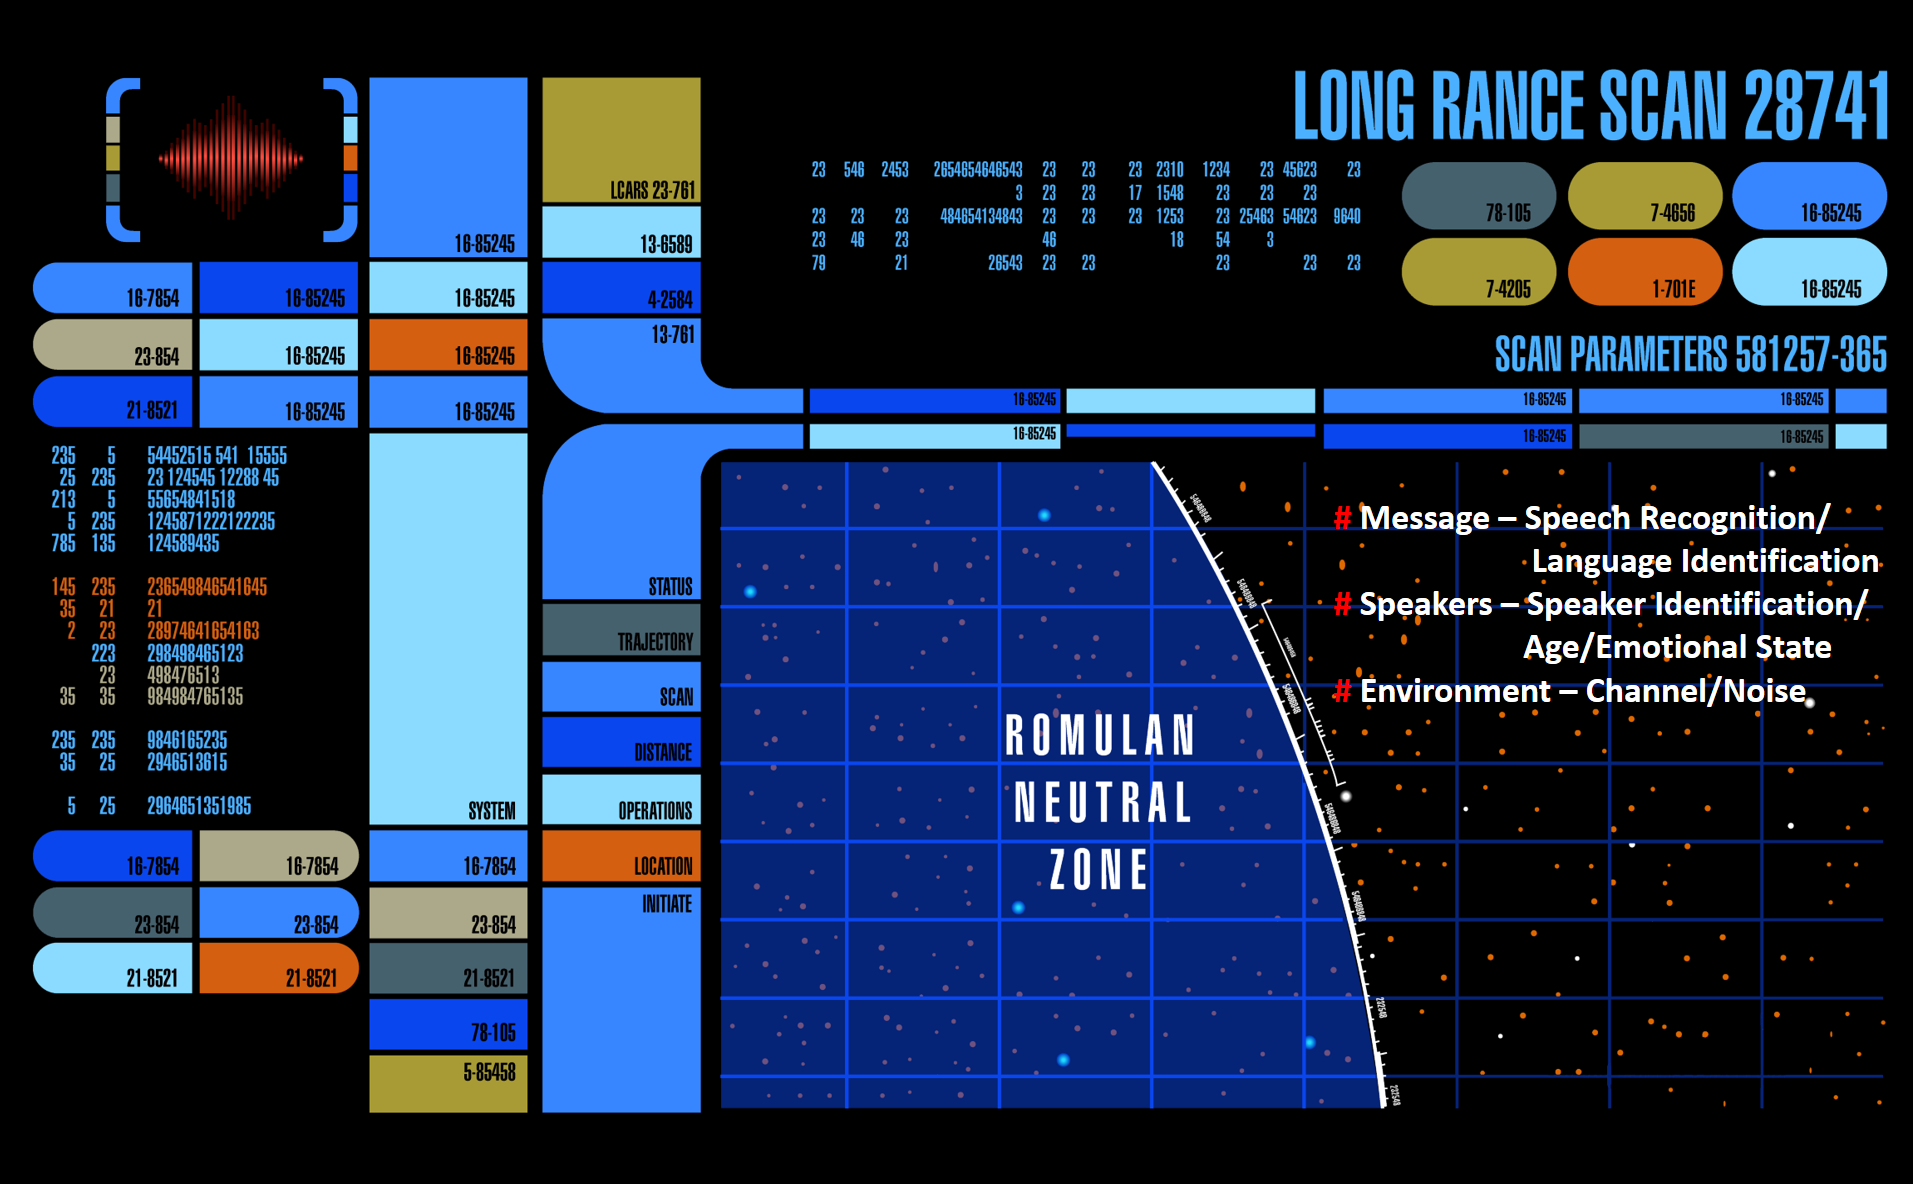
\includegraphics[height=70mm]{figures/technologies}
\end{frame}

% Show the progress from rule based to data based technologies
\begin{frame}{The march to becoming ubiquitous?}
\scalebox{1}{
\begin{tabular}{r |@{\foo} l}

{\color{red}1877} & Thomas Edison's phonograph\\
{\color{red}1936} & First electronic speech synthesizer - the Voder\\
{\color{red}1962} & IBM's Shoebox - understands up to 16 spoken\\
{\color{red}1976} & DARPA program - CMU's 1K word recognizer - Harpy\\
{\color{orange}1980} & HMMs - IBM's 20K word recognizer - Tangora\\
{\color{orange}1990} & Dragon Dictate, consumer based speech recognition\\
{\color{orange}1993} & CMU's Sphinx-II LVCSR system\\
{\color{orange}1996} & IBM's MedSpeak commercial LVCSR system\\
{\color{ForestGreen}2007} & Microsoft's Windows Vista with speech recognition\\
{\color{ForestGreen}2008} & Google's Voice Search for iPhone\\
{\color{ForestGreen}2011} & Apple's Siri \\
{\color{ForestGreen}2014} & Microsoft's Cortona/Amazon's Echo \\

\end{tabular}
}
\end{frame}

% Show the progress in building technologies across languages
\begin{frame}{In how many different ways can we speak?}
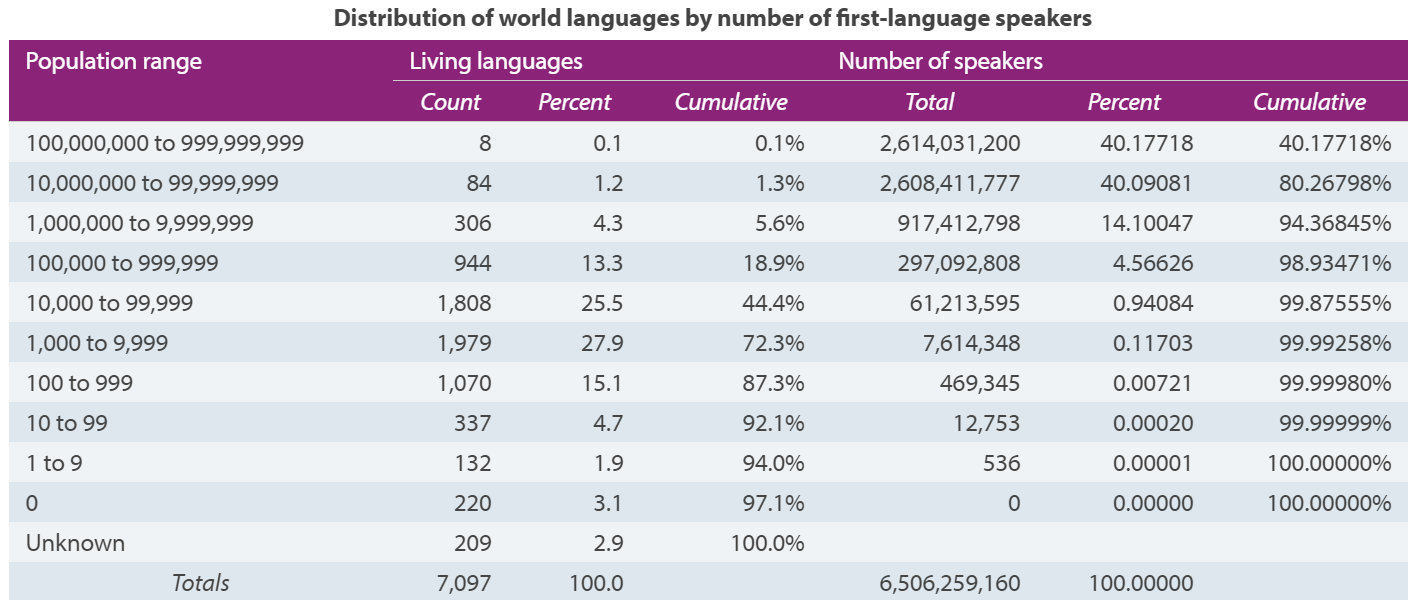
\includegraphics[height=48mm]{figures/languages}
\end{frame}

% Show the progress in building technologies across languages
\begin{frame}{Do speech technologies stand tall?}
\begin{columns}[T]
    \column{1.4in}
     \vspace{2.5cm}
     \alert{Less than 4\%} of the language space has been covered!
     \column{2.8in}
     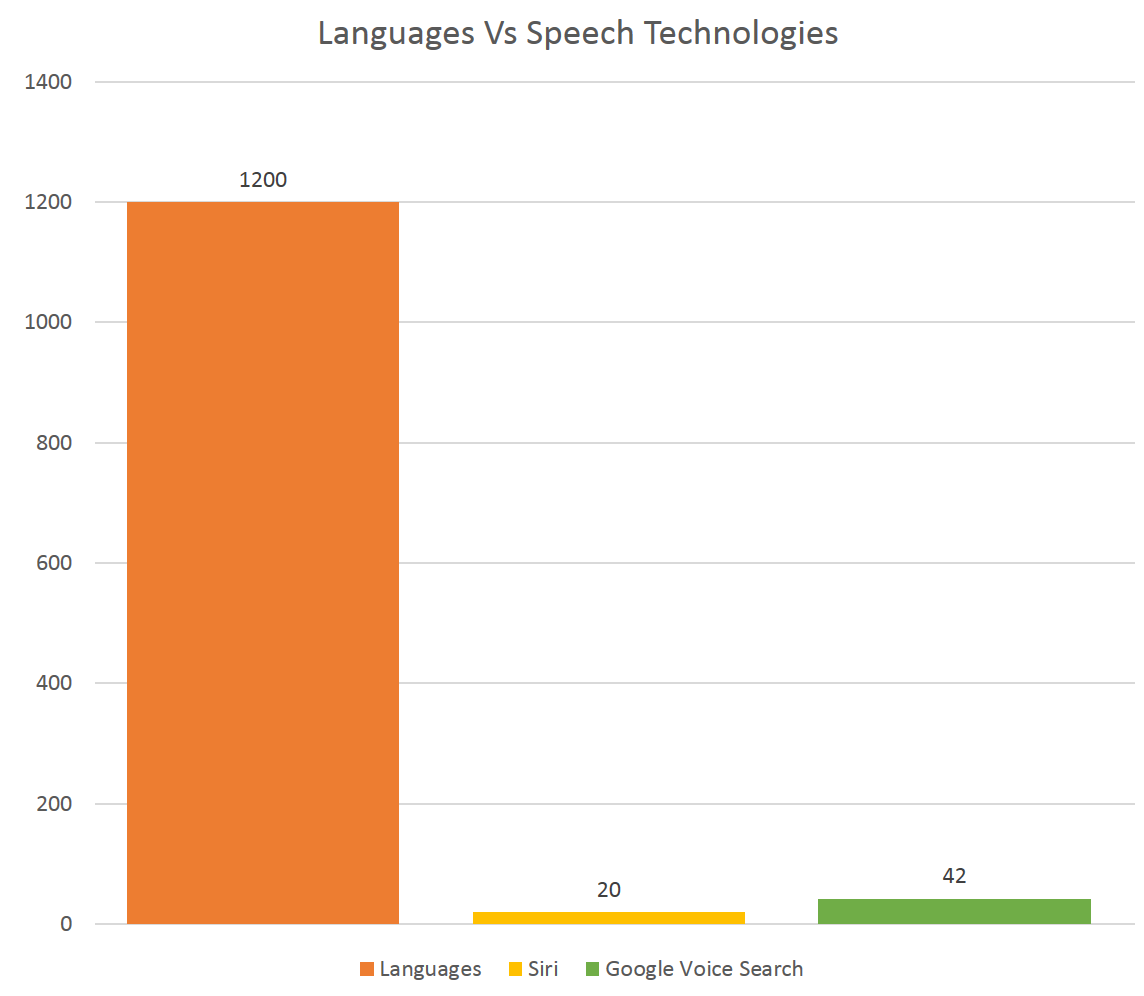
\includegraphics[height=68mm]{figures/lan_tech}
  \end{columns}
\end{frame}

% Show the progress in building technologies across languages
\begin{frame}{For a given language, New Speech Applications = New Domains?}

\begin{enumerate}
\item \alert{Applications}
\begin{enumerate}
  \item Mobile phone applications - voice search
  \item IVR applications/Call centers
  \item Dictation - Medical Transcription
  \item Surveillance - Military/Law enforcement
  \item In-car/at-home appliances
  \item Education/Accessibility
  \item Transcription - Court reporting
  \item Robotics/Gaming
\end{enumerate}
\item \alert{Noise distortions} to speech input of existing applications
\begin{enumerate}
  \item Additive Noise
  \item Convolutive Noise
\end{enumerate}
\item Every \alert{new} speech recognition deployment!
\end{enumerate}
\end{frame}

\begin{frame}{Dealing with New Languages and Domains}
\begin{columns}[T]
\column{2in}
\centering
{\color{orange}{New Languages}}
\begin{enumerate}
\item Every language is \alert{unique} although they might share many constructs with other languages
\item \alert{Separate resources} specific to the language for building ASR systems are required,
possibility to share resources across languages
\item \alert{Building a new ASR system from scratch}
\end{enumerate}
\column{2in}
\centering
{\color{ForestGreen}{New Domains}}
\begin{enumerate}
\item Domains might have specific constructs but usually involves \alert{tailoring existing resources} of a language
\item Resources from the same languages can be \alert{shared}
\item Usually \alert{an ASR adaptation problem} rather than building from scratch
\end{enumerate}
\end{columns}
\end{frame}

\begin{frame}{What's under the hood for ASR?}
\begin{enumerate}
\item Automatic speech recognition is the process of \alert{transcribing speech into text}
\item Speech recognition systems solve this task in a probabilistic setting using five key
components: \alert{a feature extraction module, an acoustic model, a pronunciation dictionary, a language model
and a search module.}
\end{enumerate}
\end{frame}

\begin{frame}{What's under the hood for ASR?}
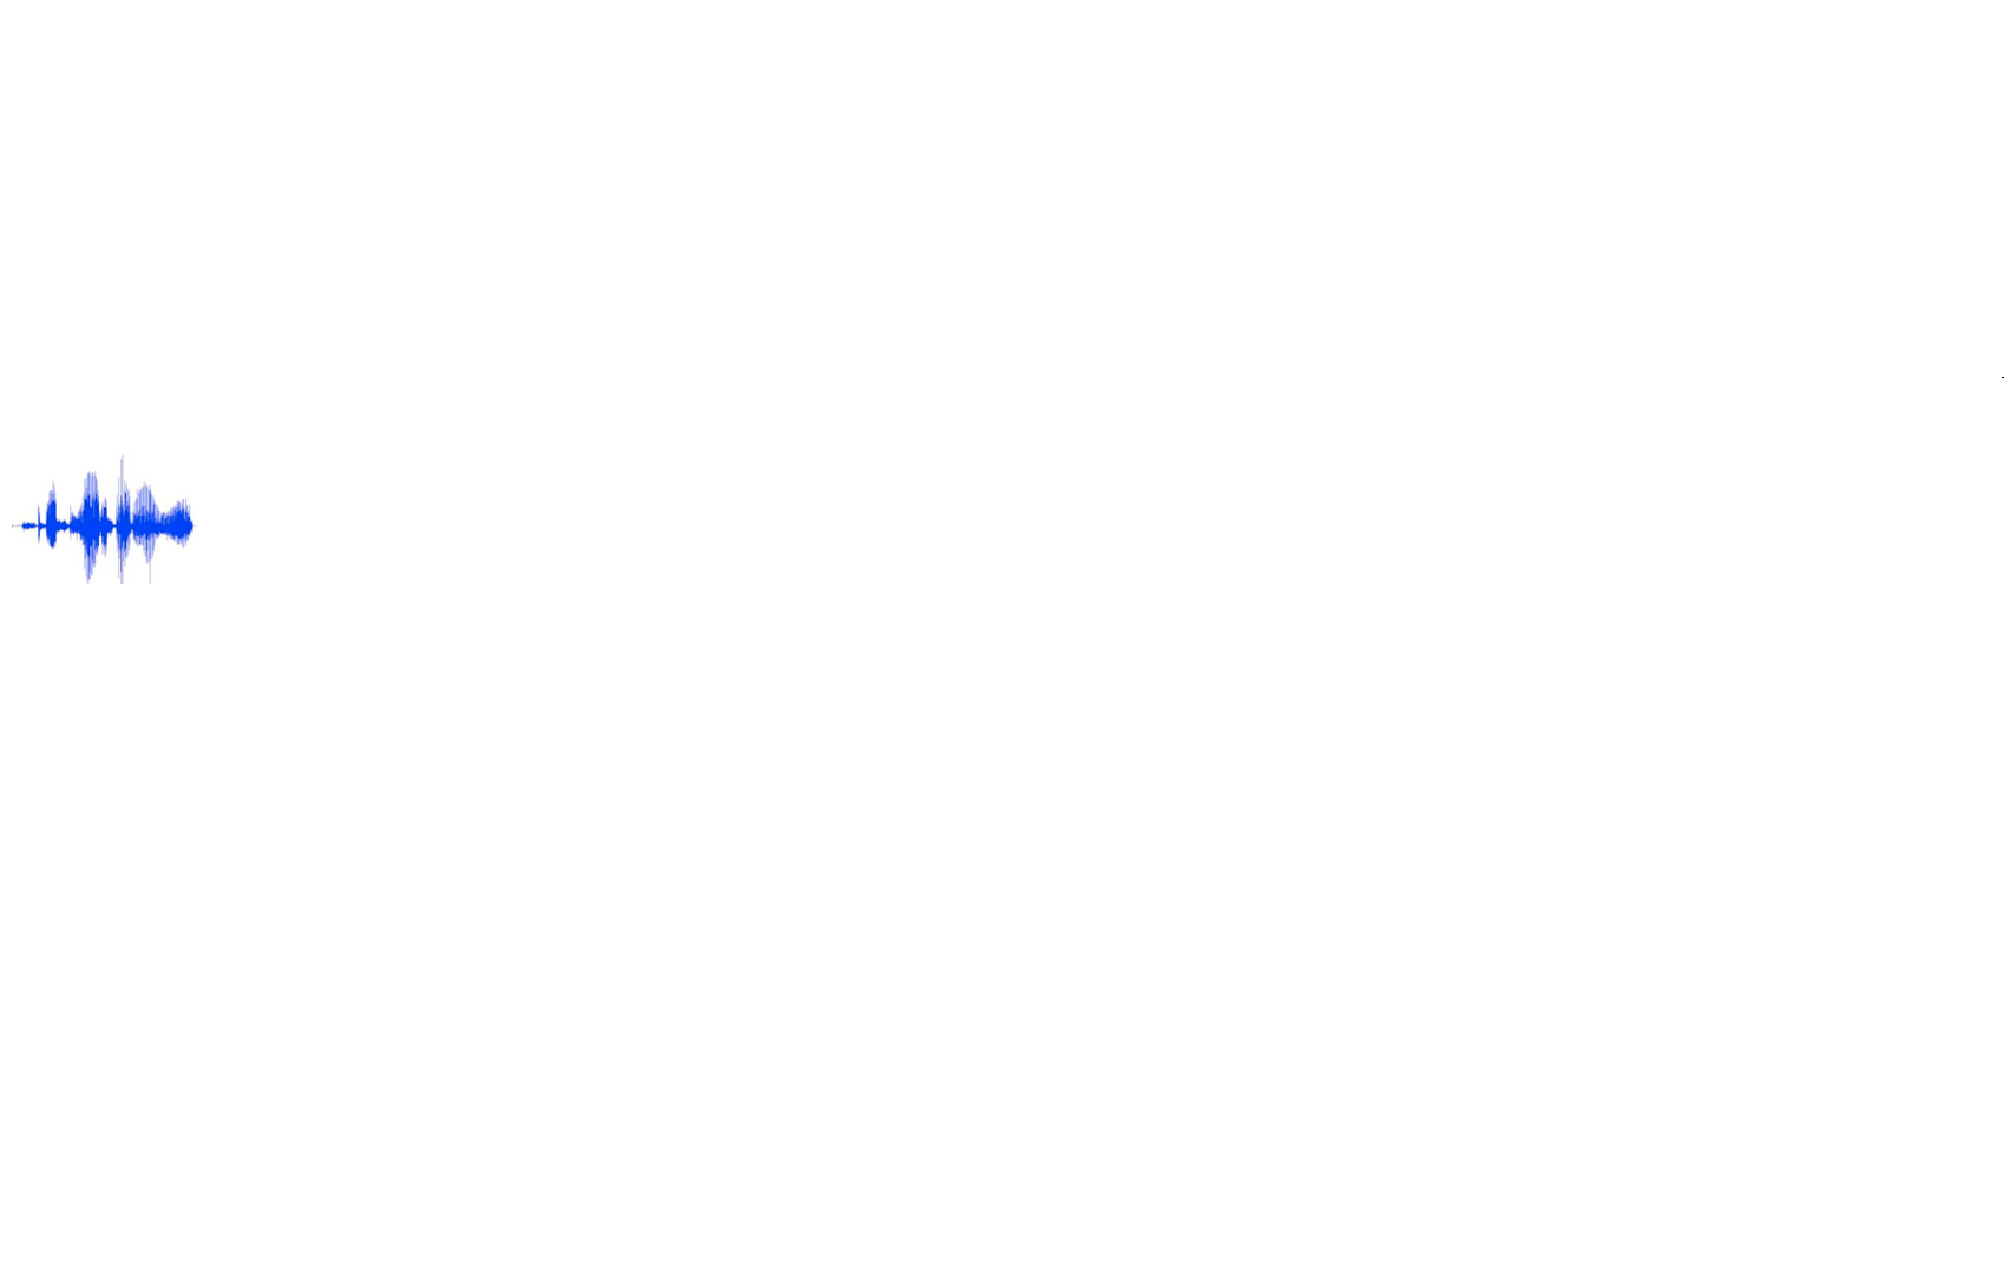
\includegraphics[height=77mm]{figures/ASR1}
\end{frame}

\begin{frame}{What's under the hood for ASR?}
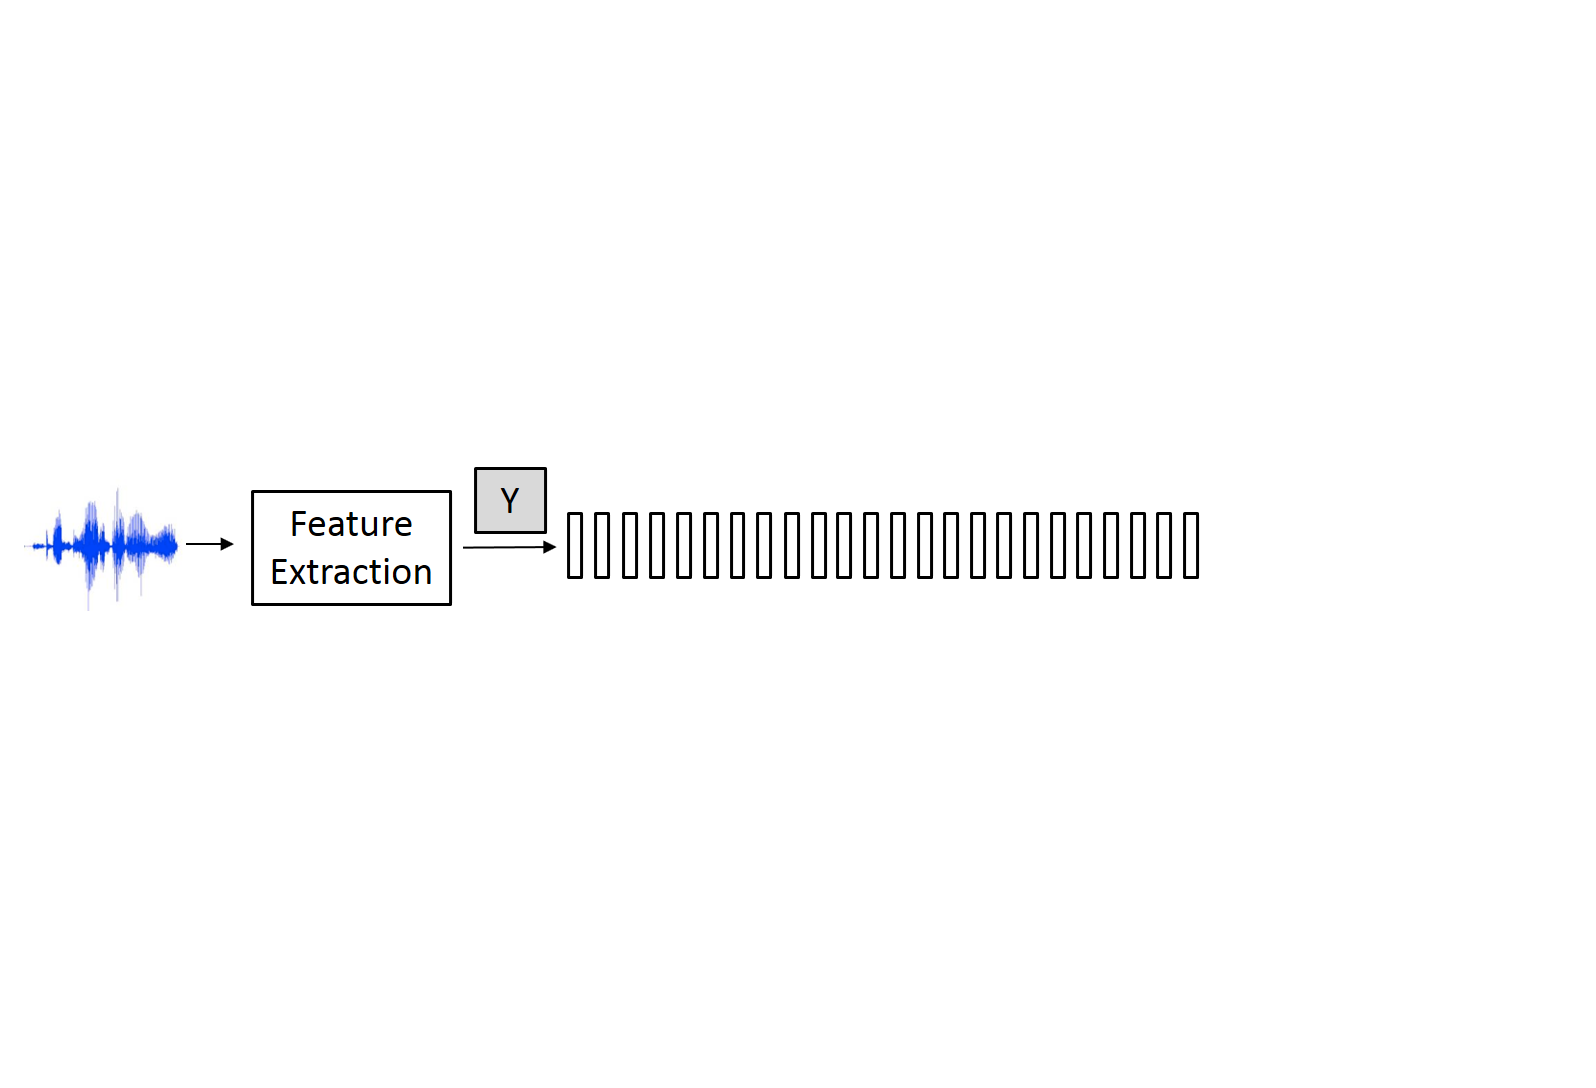
\includegraphics[height=77mm]{figures/ASR2}
\end{frame}

\begin{frame}{What's under the hood for ASR?}
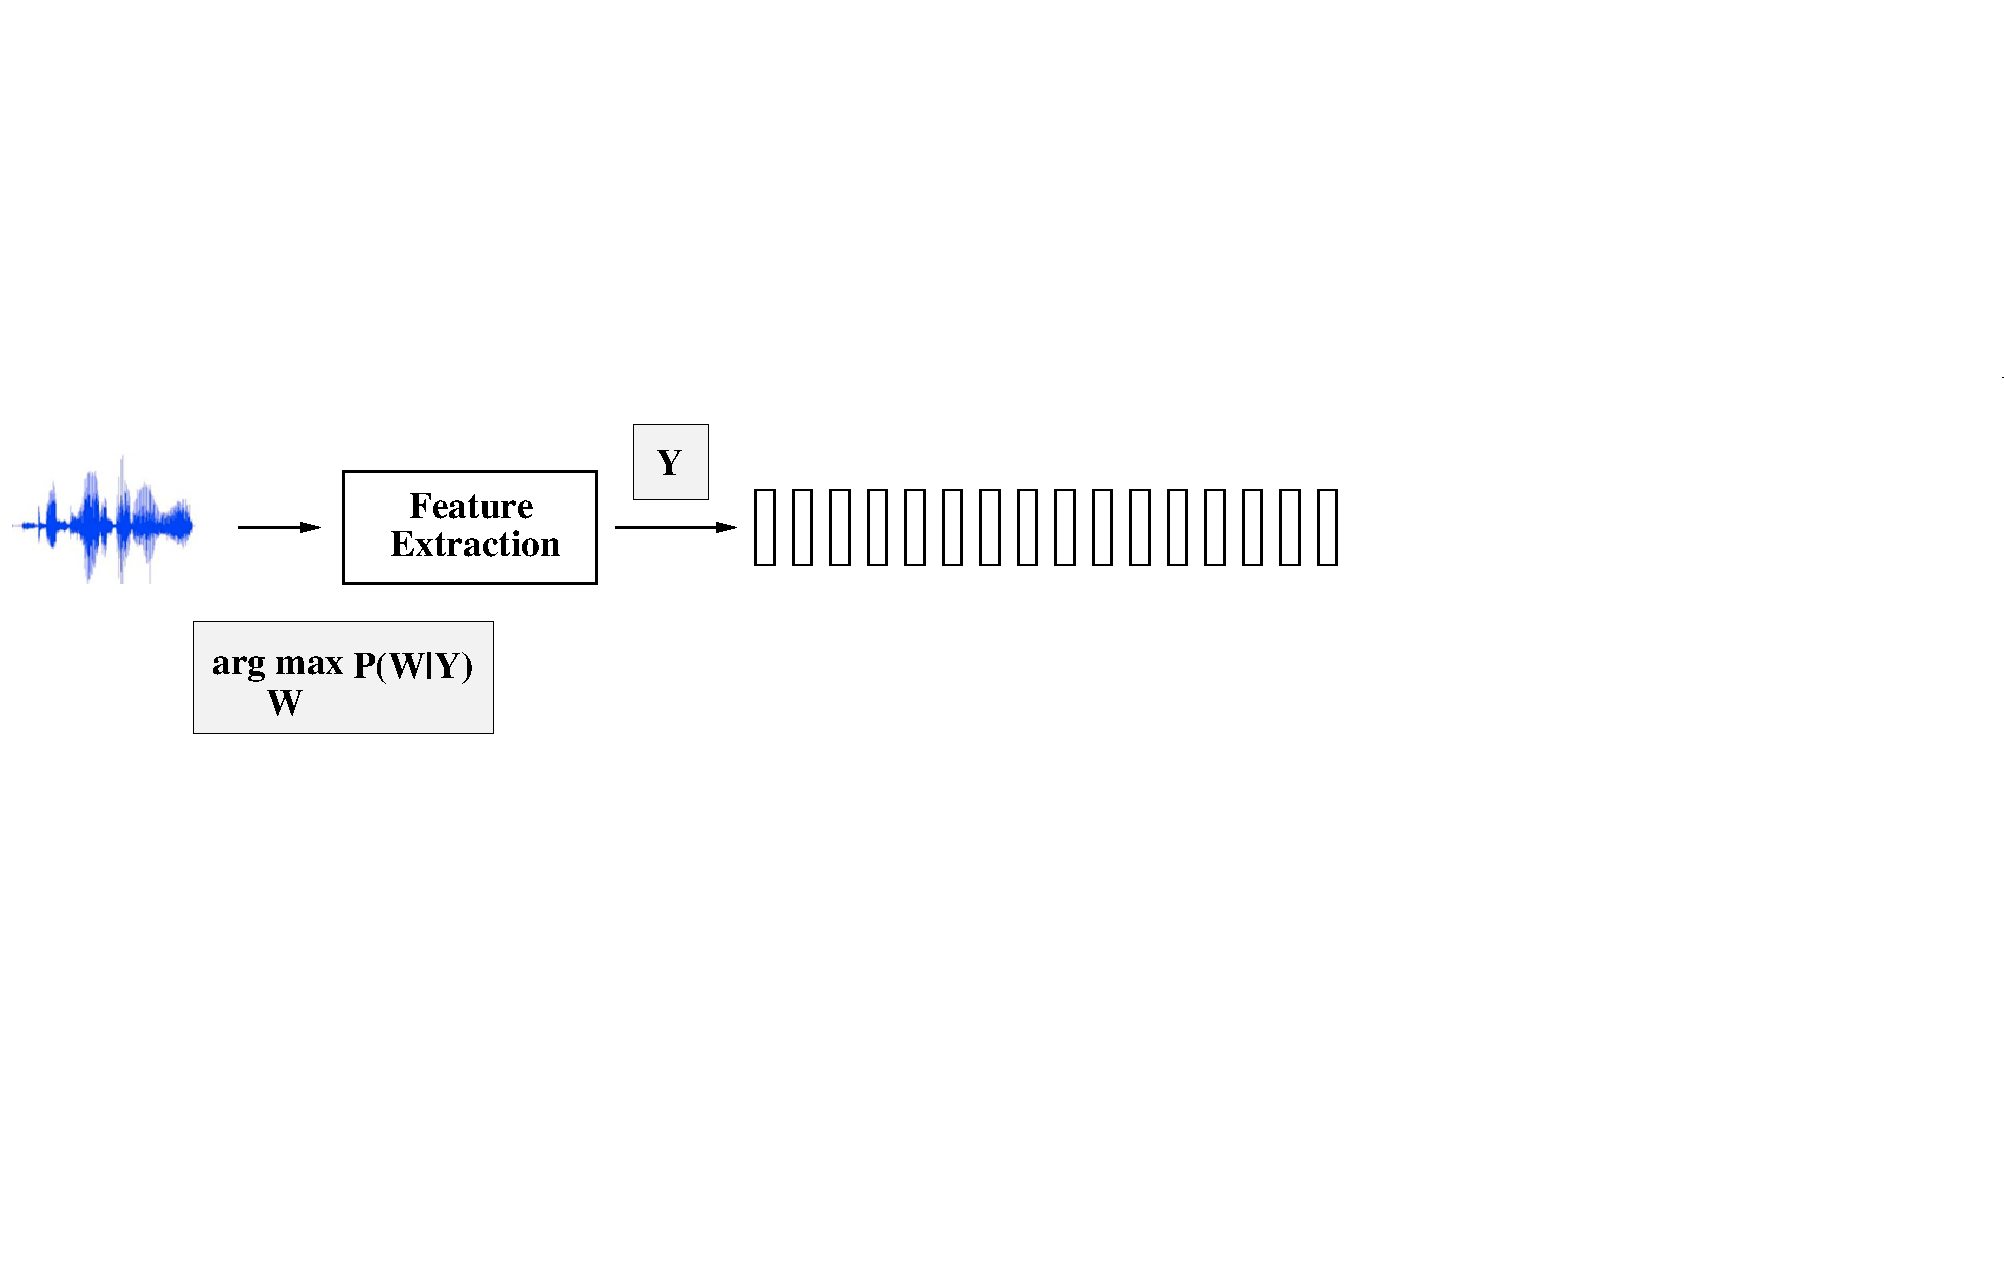
\includegraphics[height=77mm]{figures/ASR3}
\end{frame}

\begin{frame}{What's under the hood for ASR?}
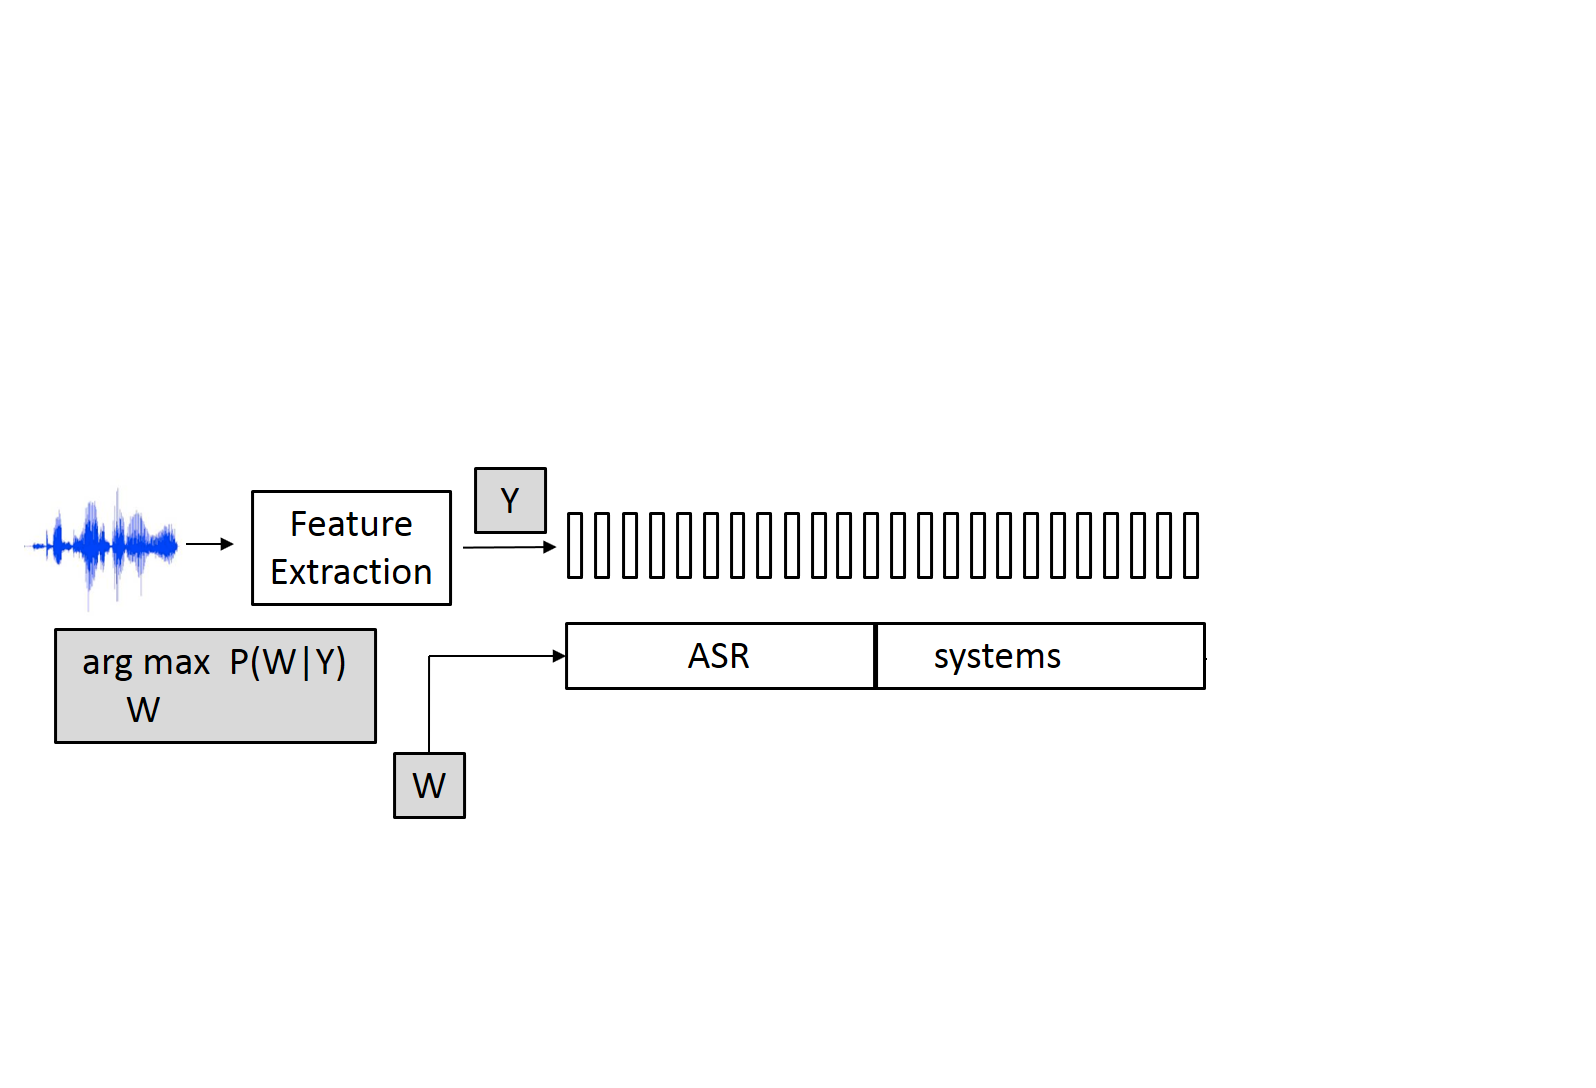
\includegraphics[height=77mm]{figures/ASR4}
\end{frame}

\begin{frame}{What's under the hood for ASR?}
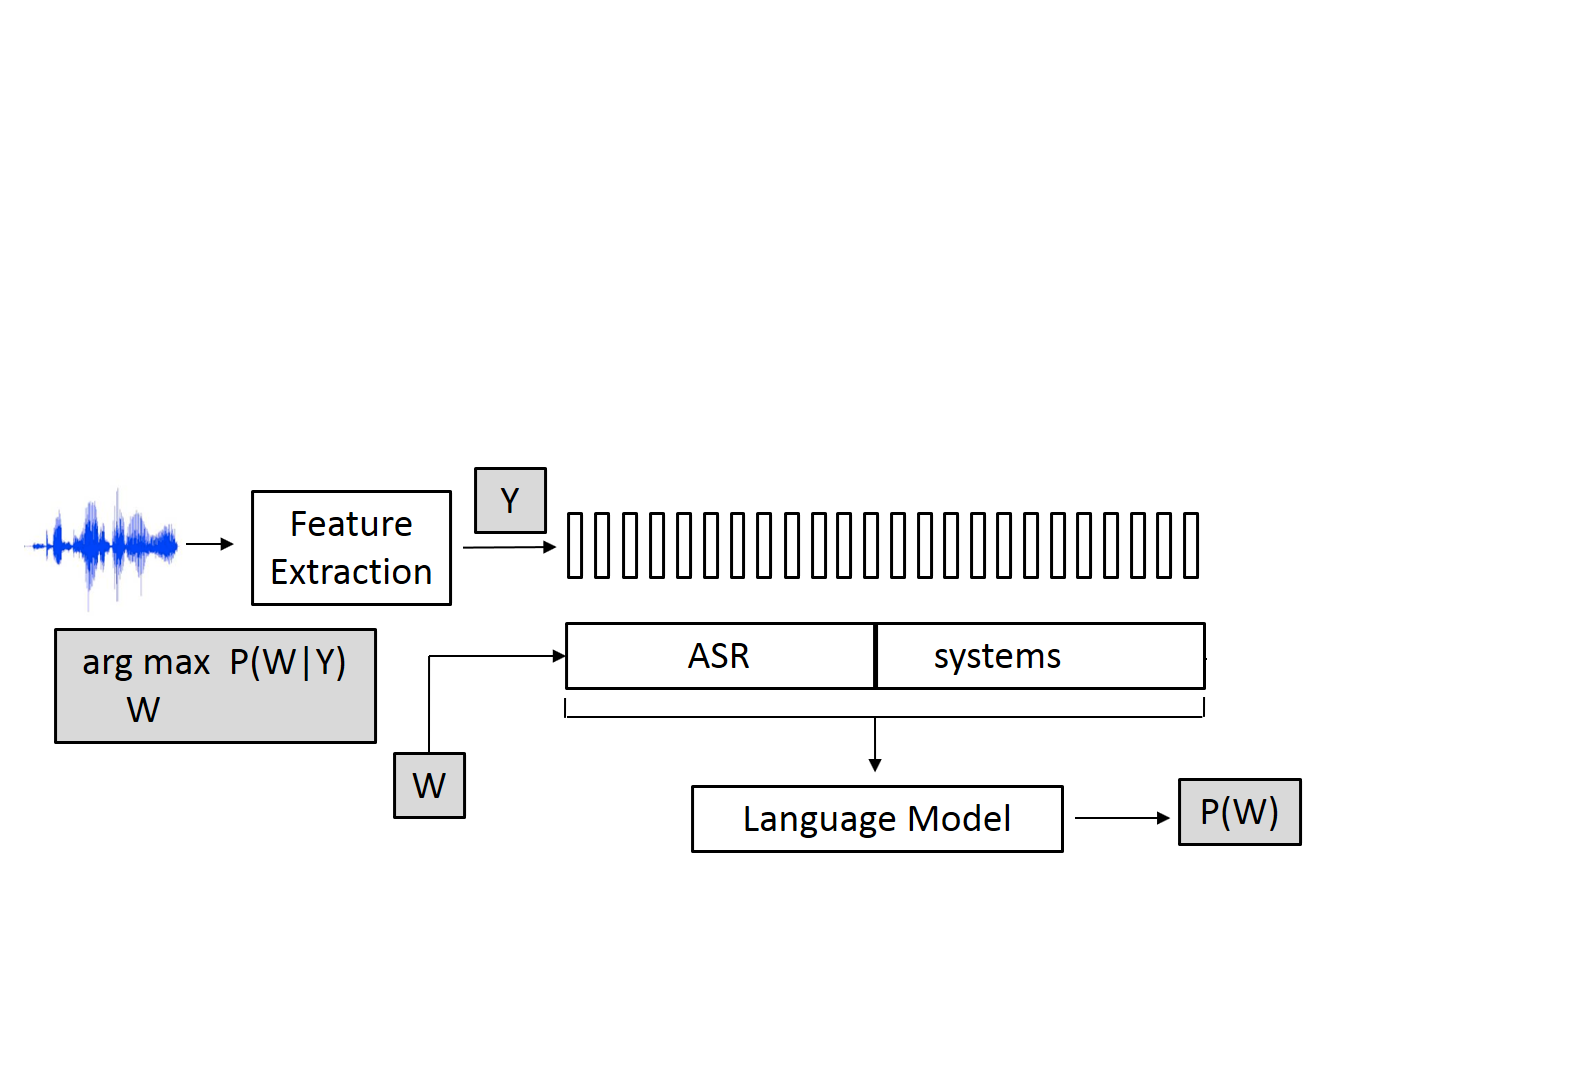
\includegraphics[height=77mm]{figures/ASR5}
\end{frame}

\begin{frame}{What's under the hood for ASR?}
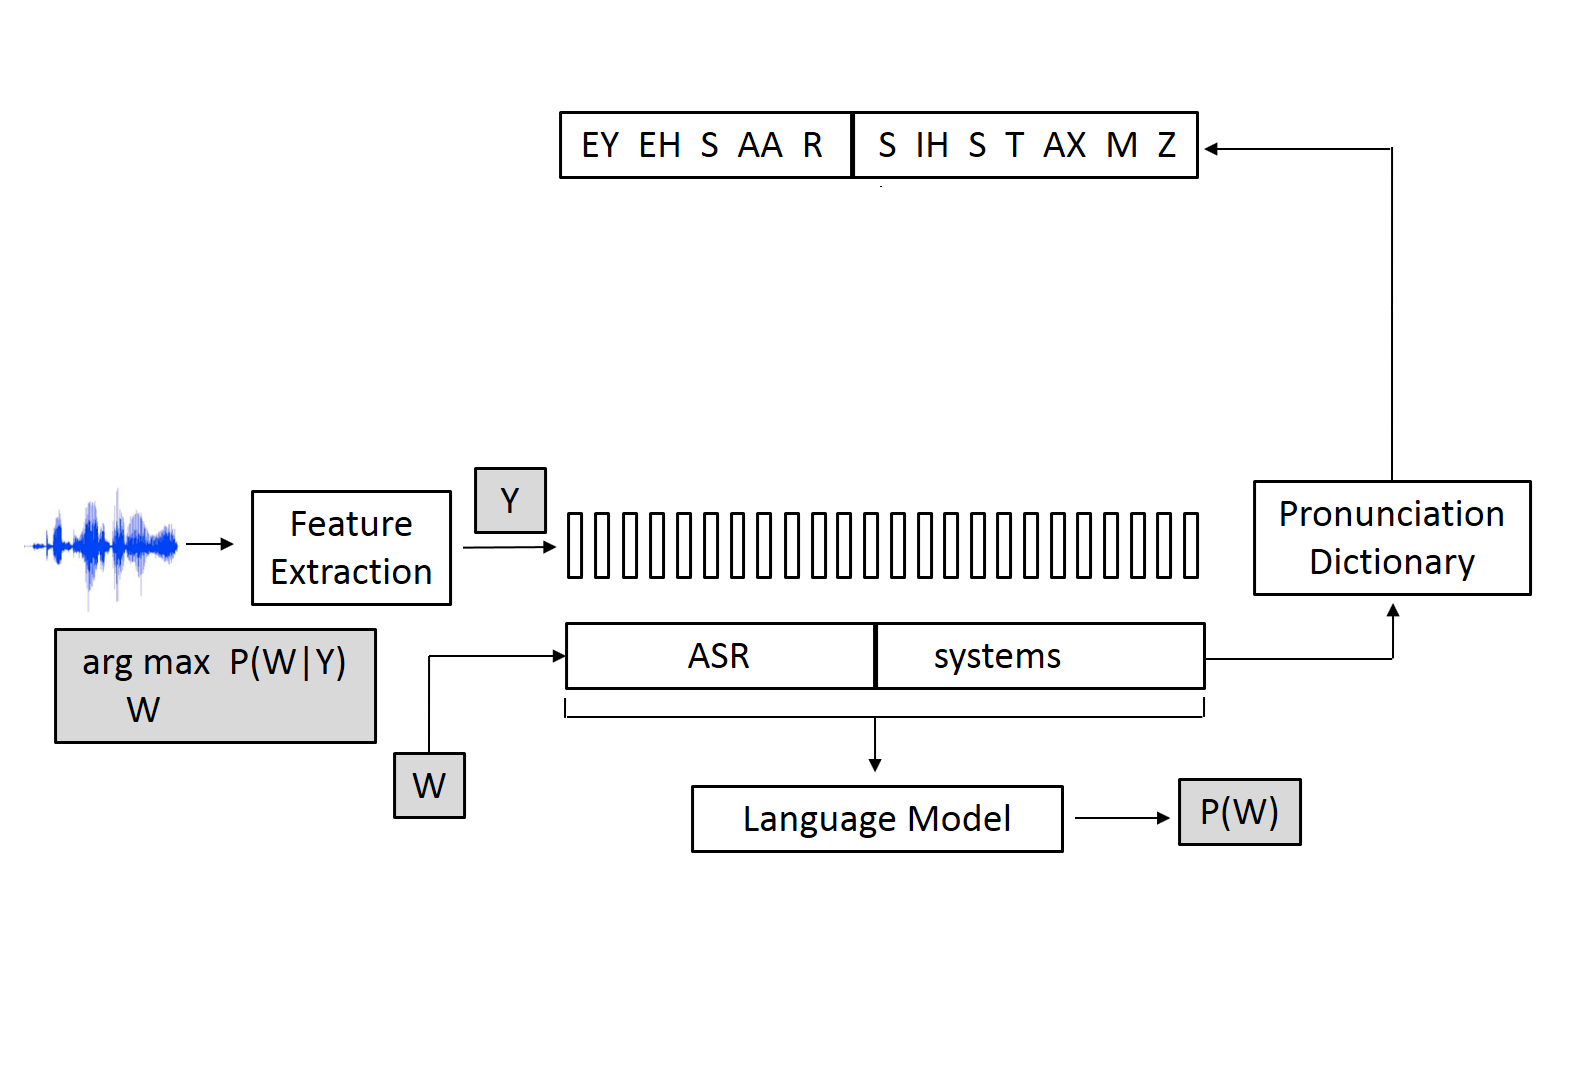
\includegraphics[height=77mm]{figures/ASR6}
\end{frame}

\begin{frame}{What's under the hood for ASR?}
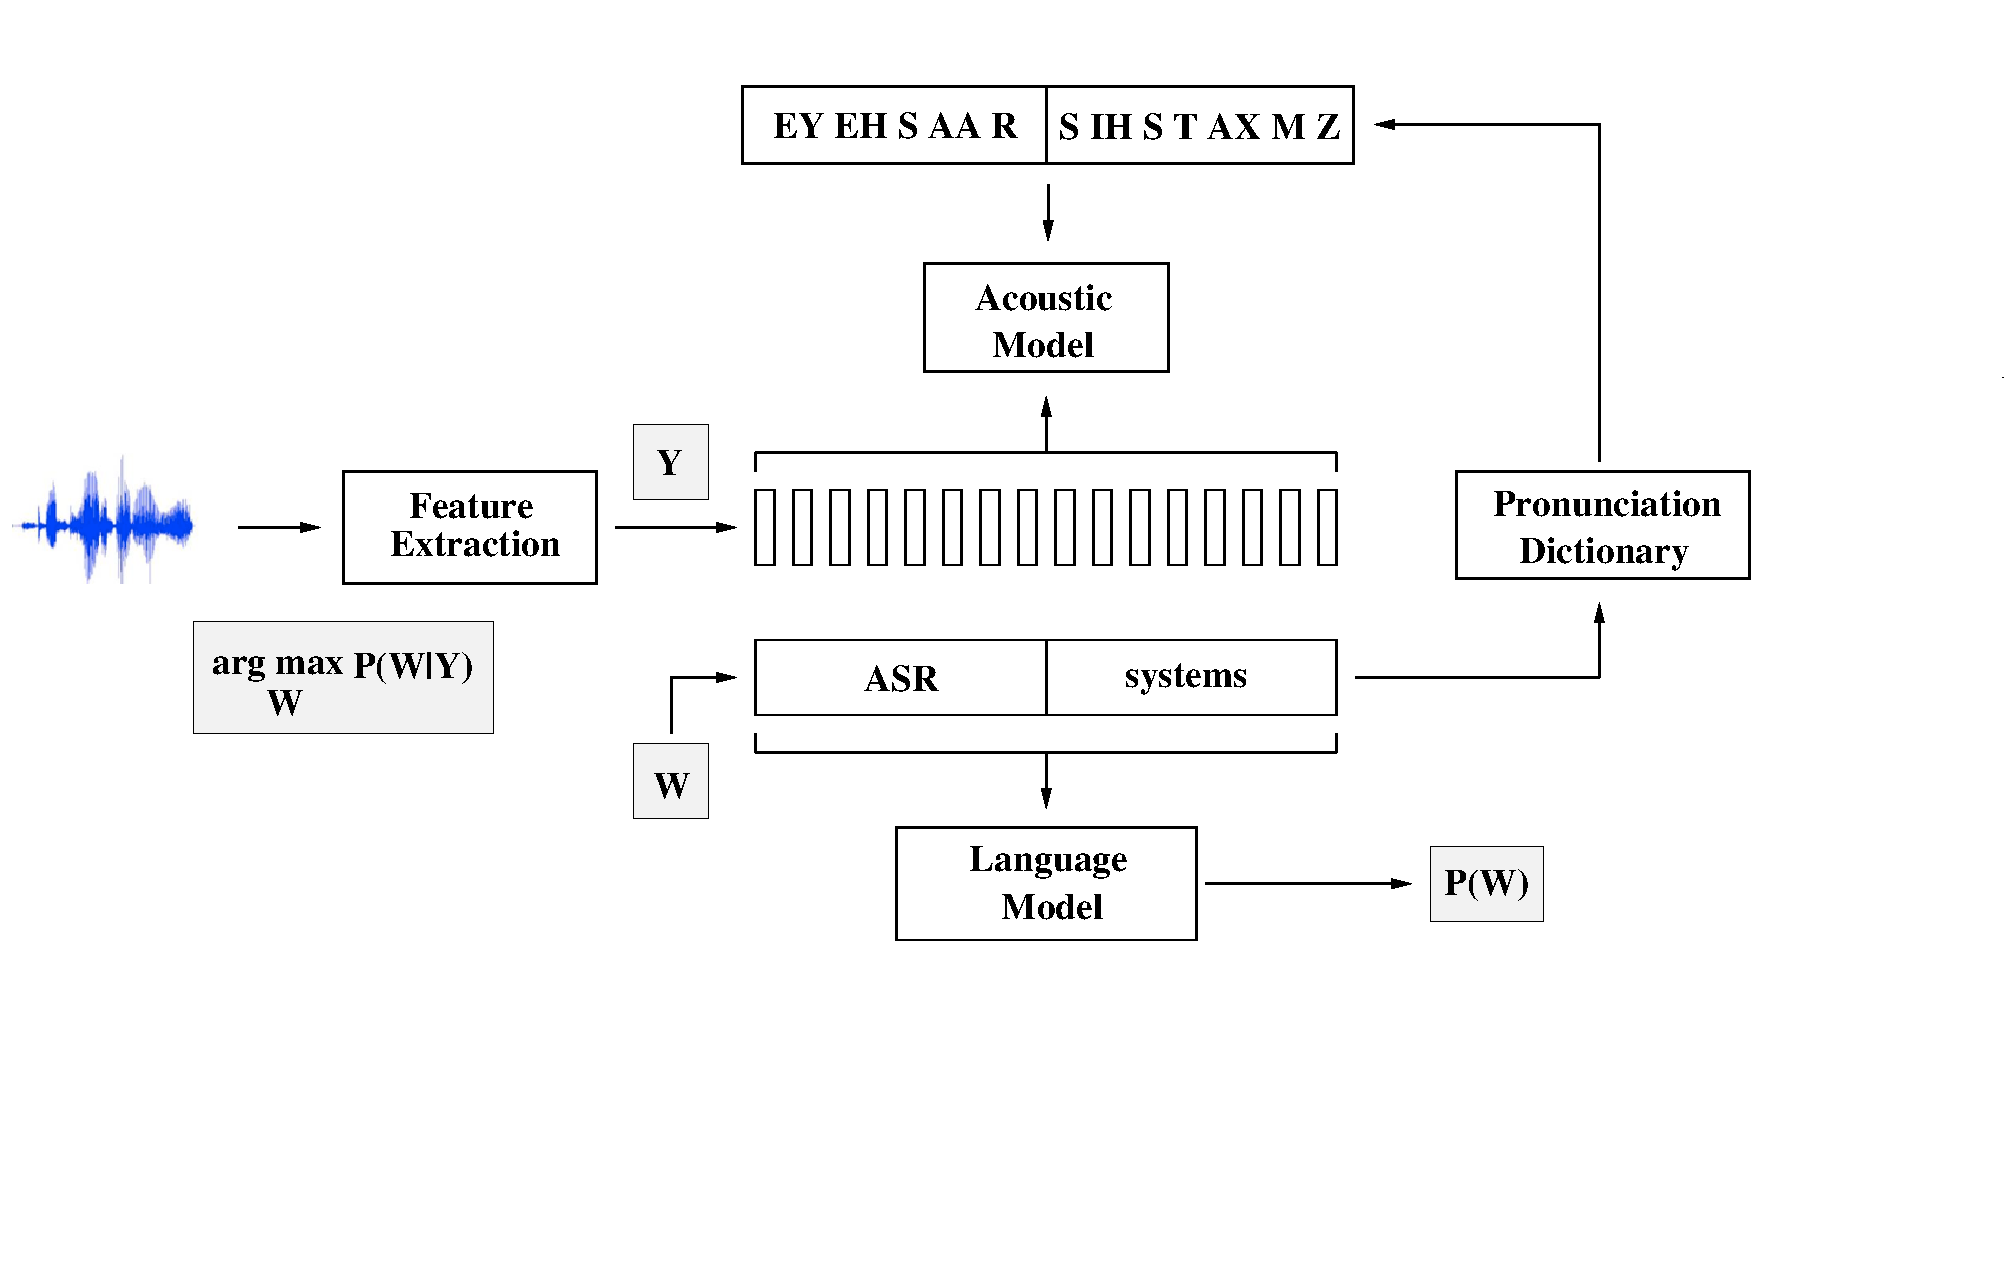
\includegraphics[height=77mm]{figures/ASR7}
\end{frame}

\begin{frame}{What's under the hood for ASR?}
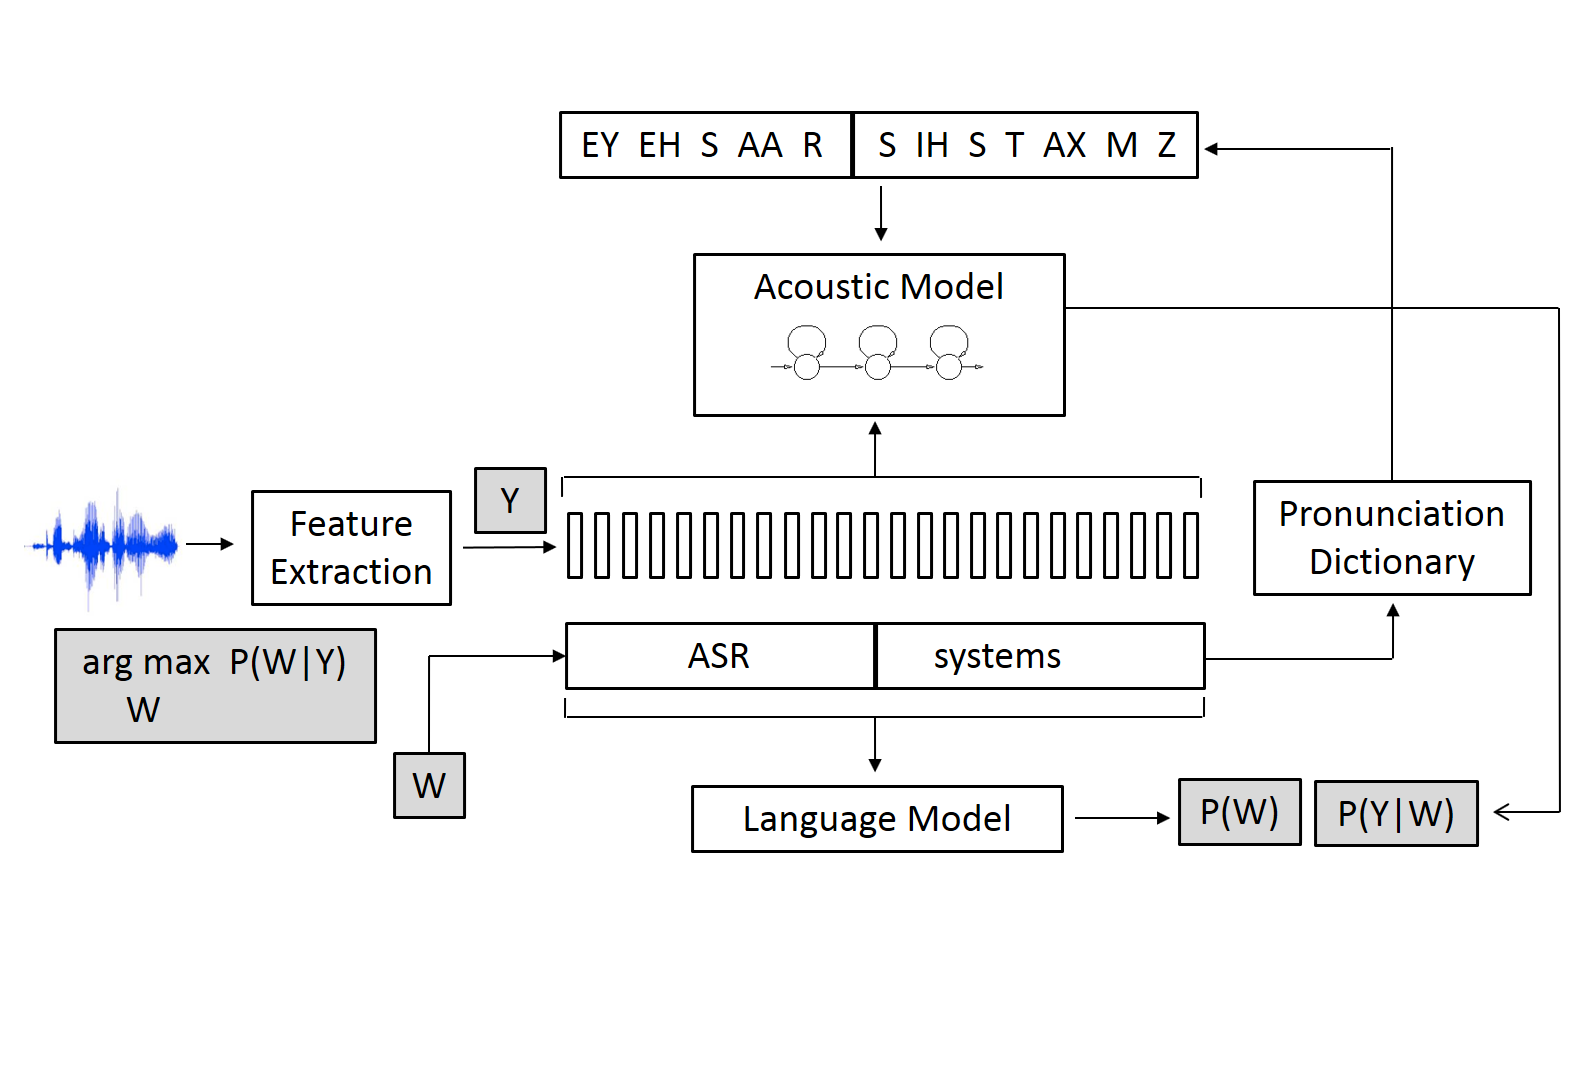
\includegraphics[height=77mm]{figures/ASR8}
\end{frame}

\begin{frame}{What's under the hood for ASR?}
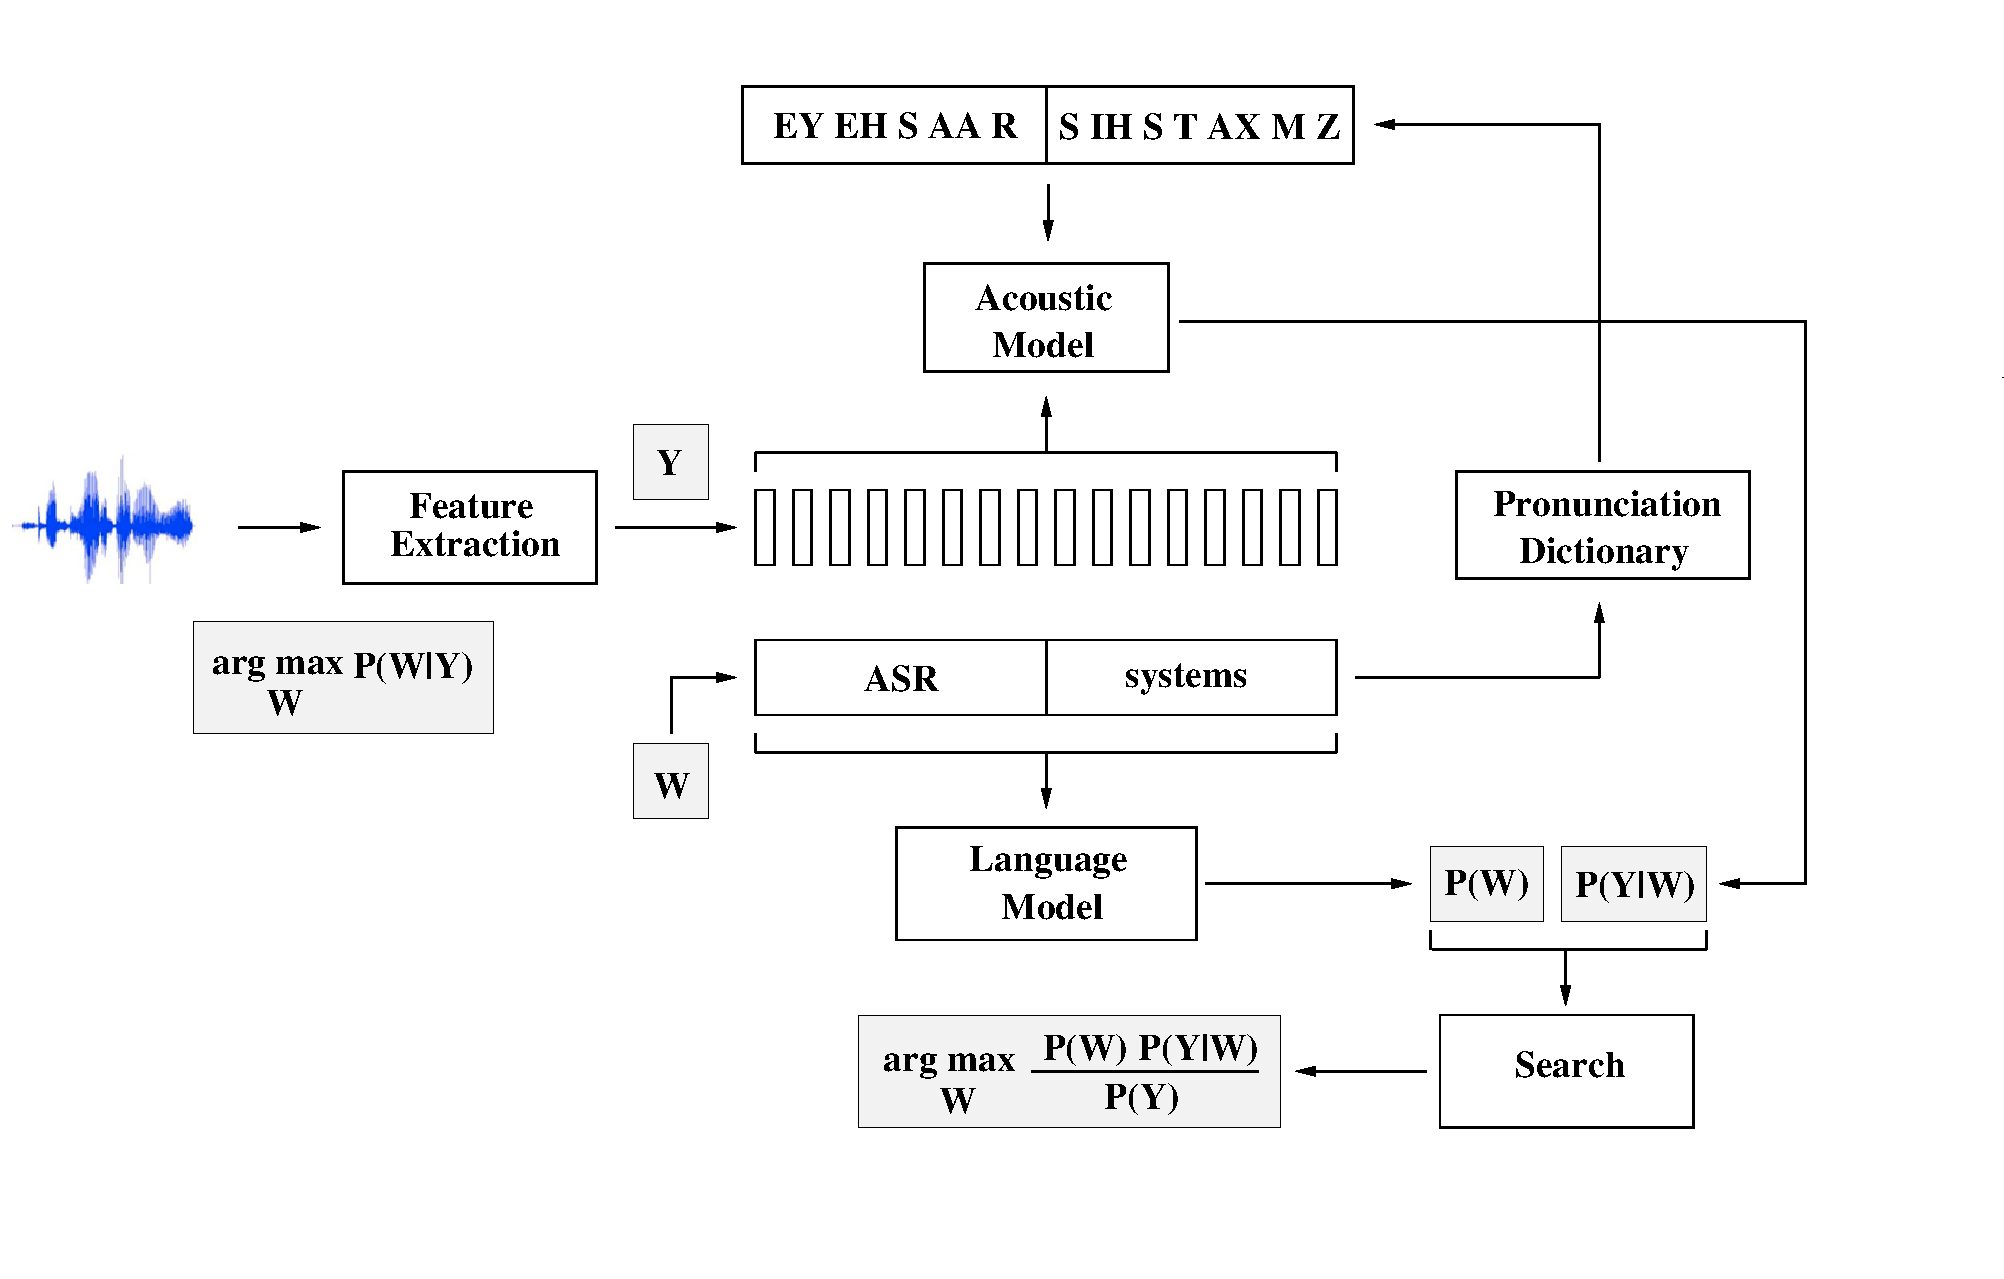
\includegraphics[height=77mm]{figures/ASR9}
\end{frame}

\begin{frame}{What's under the hood for ASR?}
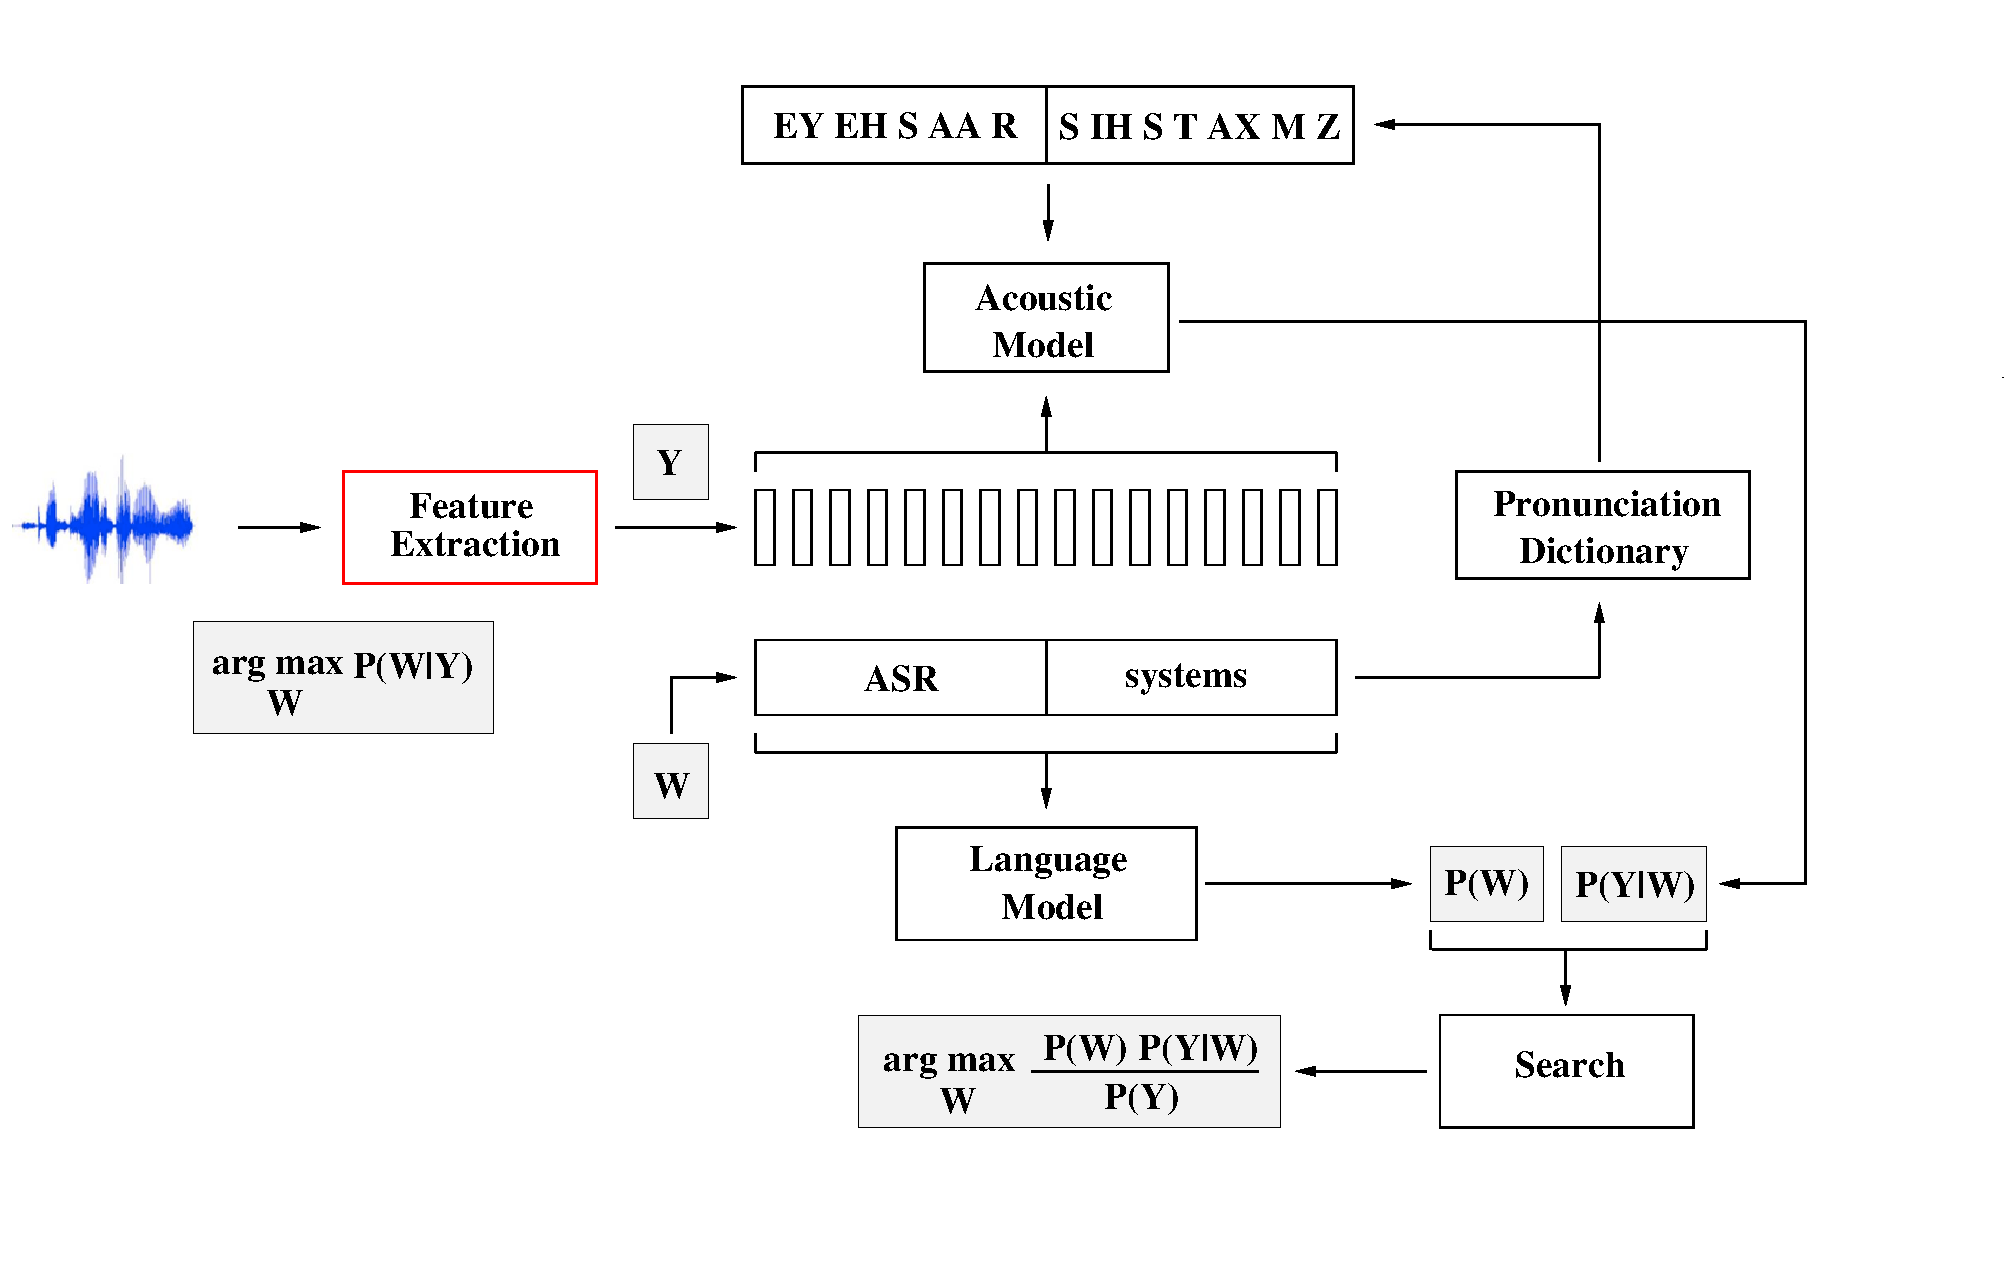
\includegraphics[height=77mm]{figures/b1}
\end{frame}

\begin{frame}{Feature Extraction - Introduction}
\begin{enumerate}
\item Why not use the speech signal directly for pattern recognition?
\begin{enumerate}
\item Speech is a \alert{time-varying non-stationary signal}
\item Information may lie in a \alert{small portion} of signal
\item May contain \alert{irrelevant information} for the application
\item Presence of \alert{noise and other distortions}
\item \alert{Size and dimensionality} of the data
\end{enumerate}
\item Need to transform the signal into lower dimensional descriptors called \alert{features}.
\end{enumerate}
\end{frame}

\begin{frame}{Feature Extraction - "Past" Techniques}
\begin{columns}[T]
    \column{2in}
	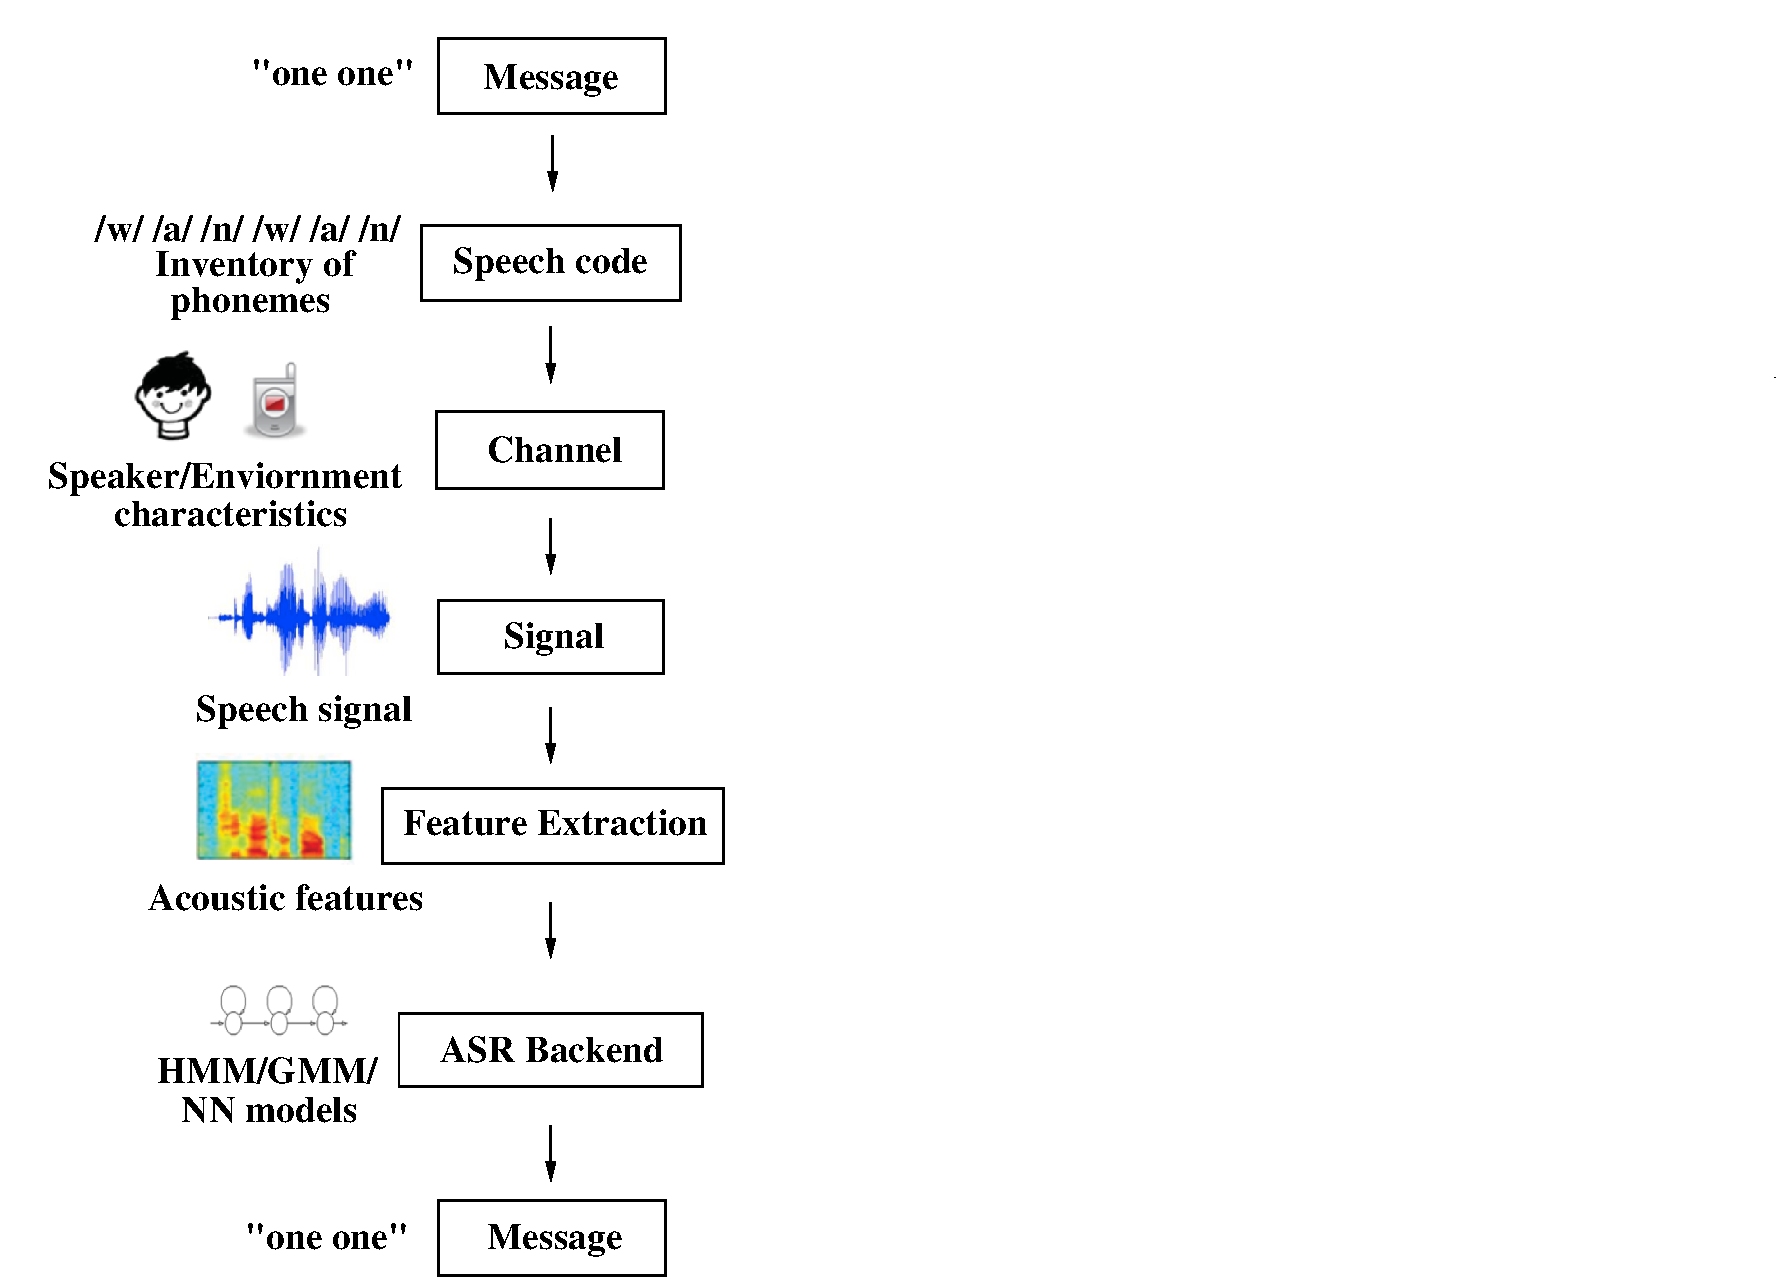
\includegraphics[height=73mm]{figures/acoustic}
     \column{2in}
	\begin{enumerate}
	\item \alert{Speech Coding Inspired Features} - Mel Spectrogram and Linear Prediction
	\item \alert{Speech Synthesis Inspired Features} - Pitch and Prosody
	\item \alert{Long Contextual Features} - Delta Processing, RASTA Filtering and Modulation Features
        \item \alert{Normalization Techniques} - Cepstral Mean Normalization and Spectral Subtraction
	\end{enumerate}
\end{columns}
\end{frame}

\begin{frame}{Feature Extraction - Current Techniques}
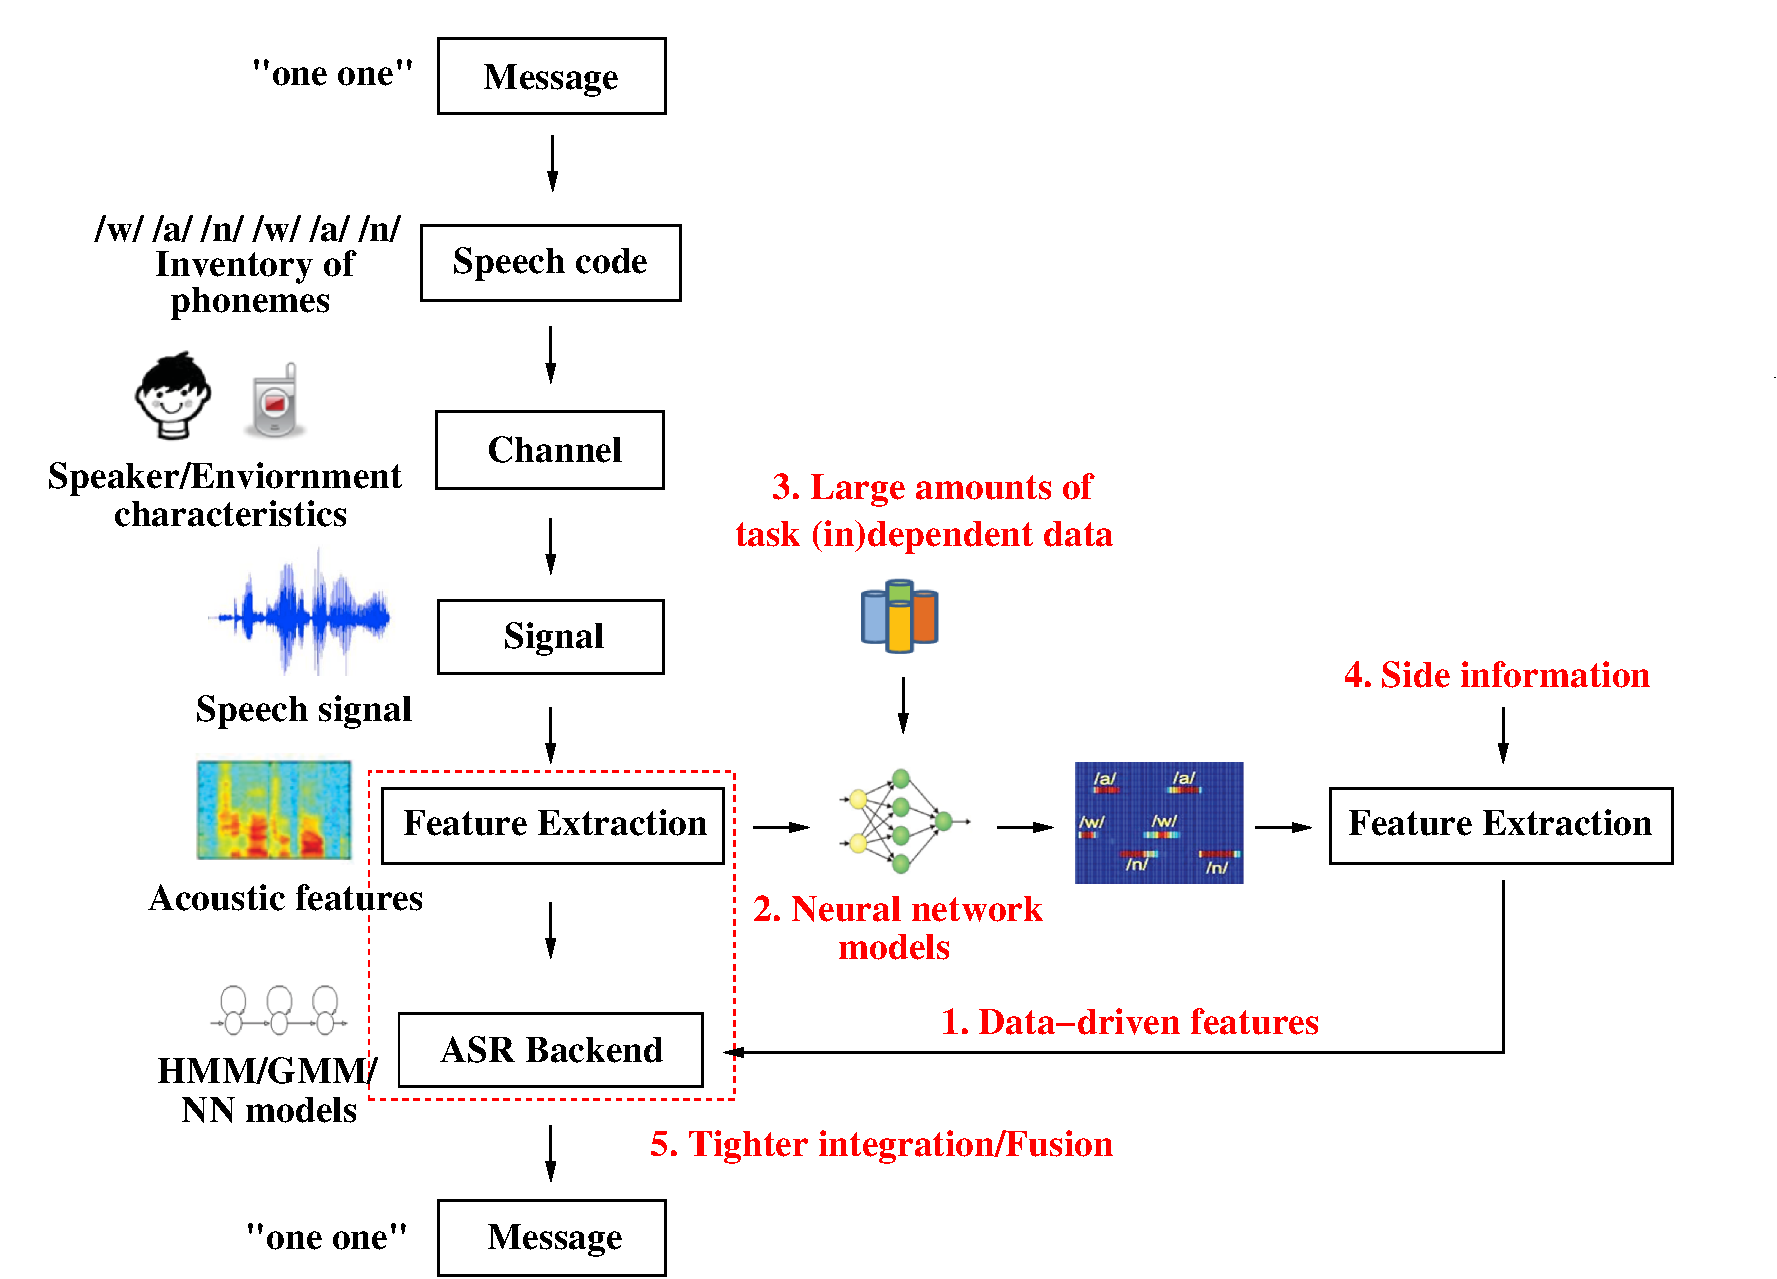
\includegraphics[height=76mm]{figures/data_driven}
\end{frame}

\begin{frame}{What's under the hood for ASR?}
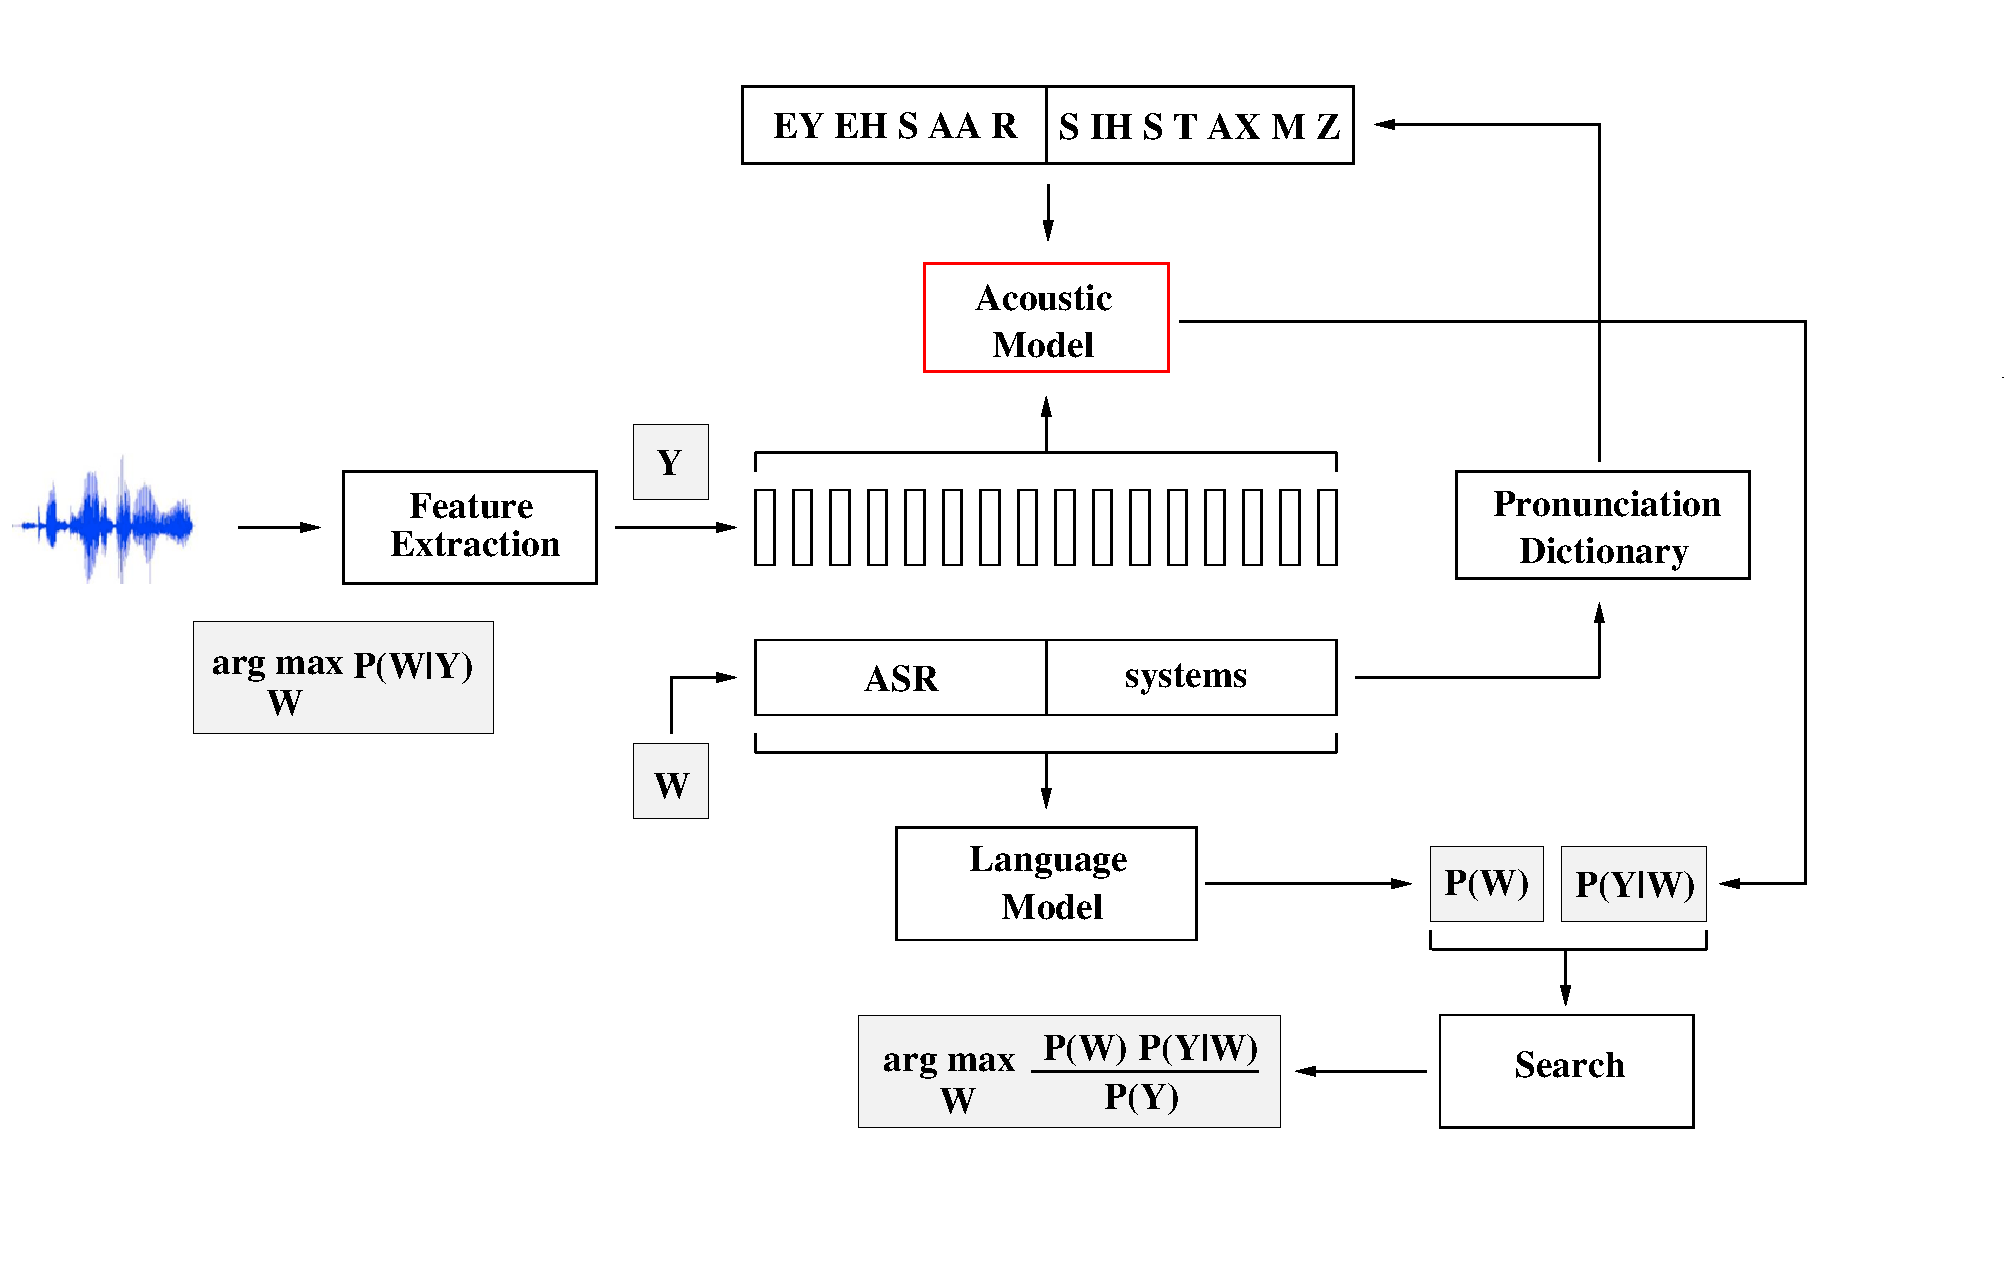
\includegraphics[height=77mm]{figures/b2}
\end{frame}

\begin{frame}{Acoustic Modeling - Introduction}
\begin{center}
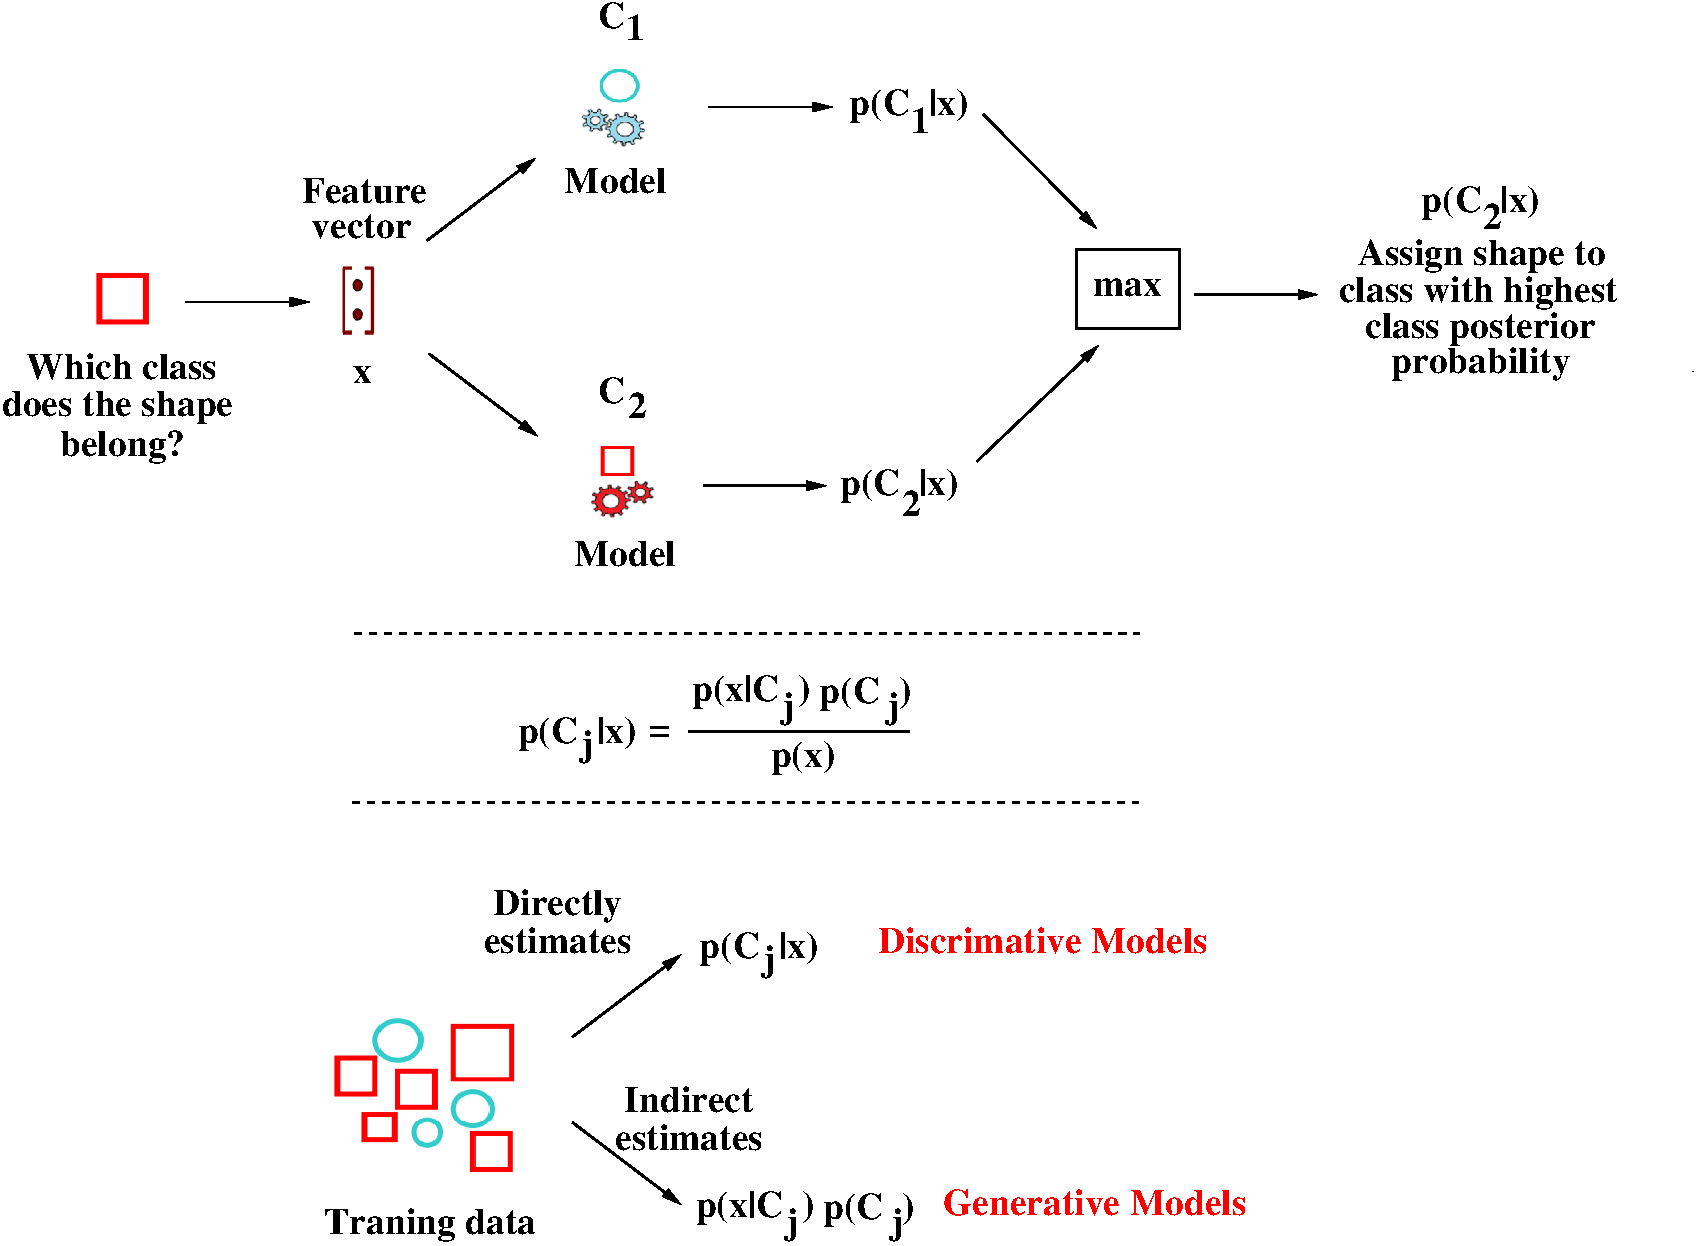
\includegraphics[height=72mm]{figures/am}
\end{center}
\end{frame}

\begin{frame}{Acoustic Modeling - "Past" Techniques}
\begin{enumerate}
\item The \alert{goal of the AM} is to provide a method of calculating the likelihood
of any feature vector sequence $Y$ given a word $w$
\item \alert{The basic \alert{sequence} model} -
\begin{enumerate}
\item To estimate this likelihood word sequences are decomposed into basic sound units
called phones
\item Each individual phone is represented using a Hidden Markov Model (HMM) - a state machine with 
a number of states connected with arcs in a left-right topology.
\item Each state models the distribution of acoustic vectors with Gaussian mixture models.
\item HMM algorithms: Likelihood computation (forward algorithm), most probable state sequence (Viterbi algorithm), 
estimating parameters (EM algorithm)
\end{enumerate}
\item \alert{Improvements to the basic model} -
\begin{enumerate}
\item Modeling - Context-dependent models, Tied mixture models, state clustering, phonetic decision trees
\item Training criteria - MLE, MMIE, MPE for training HMM-GMM based systems
\end{enumerate}
\end{enumerate}
\end{frame}

\begin{frame}{Acoustic Modeling - "Past" Techniques}
\begin{center}
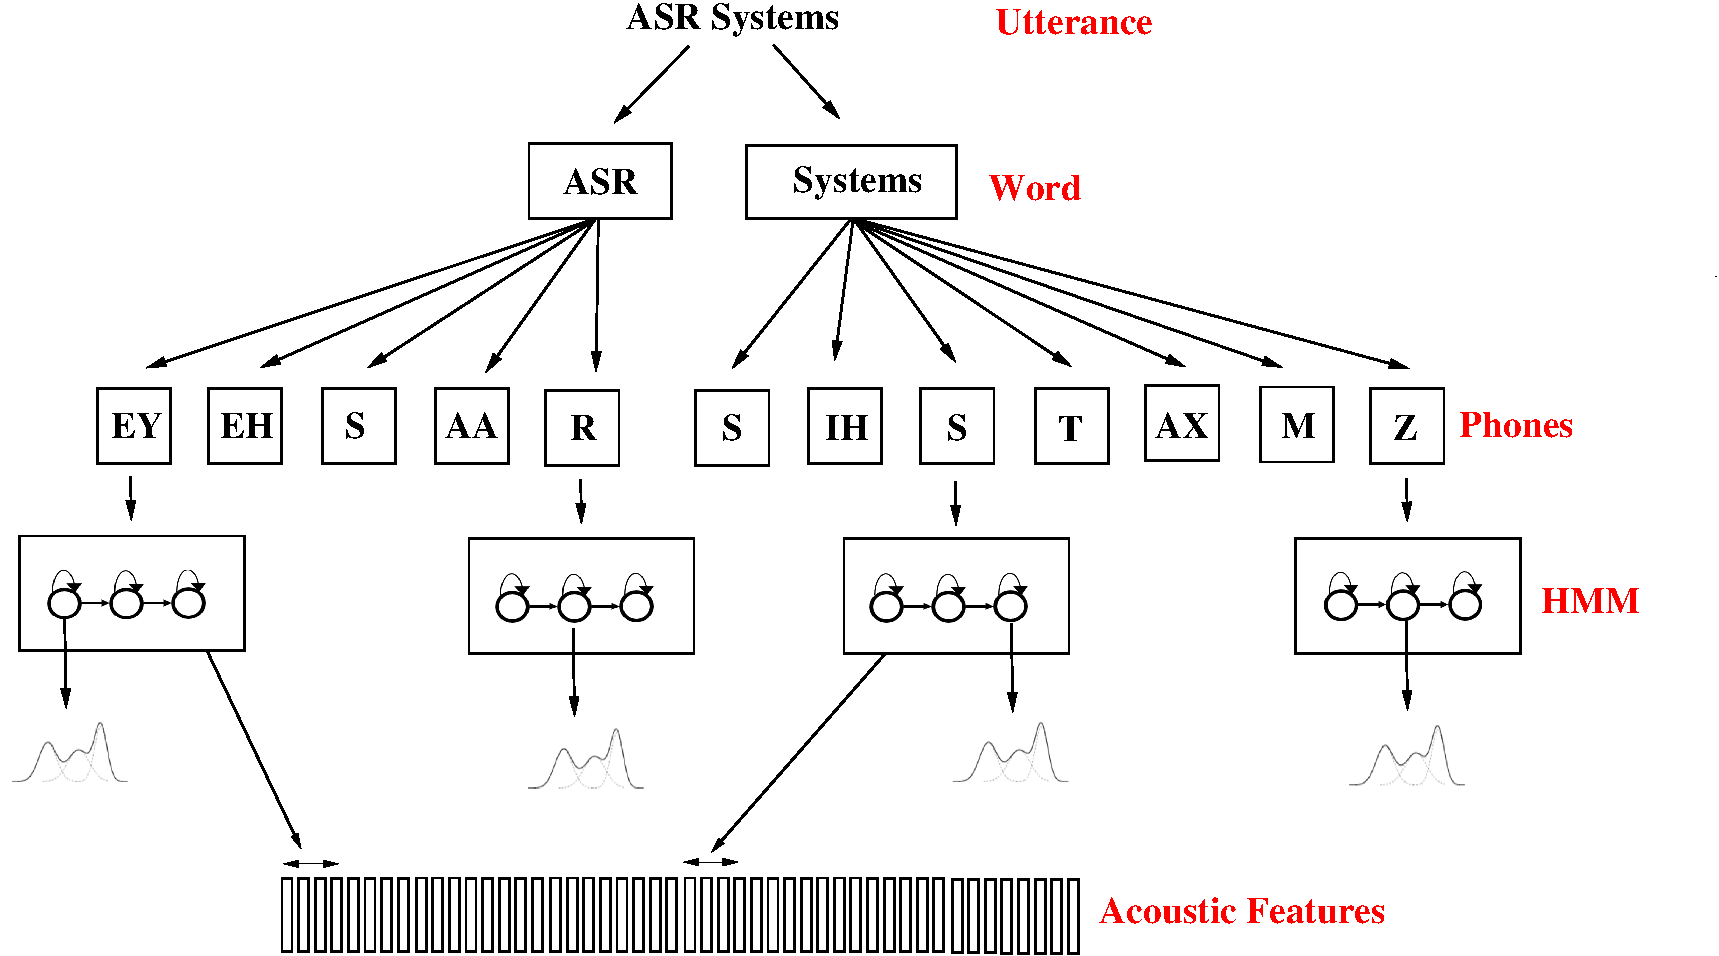
\includegraphics[height=65mm]{figures/am-gmm}
\end{center}
\end{frame}

\begin{frame}{Acoustic Modeling - Current Techniques}
\begin{center}
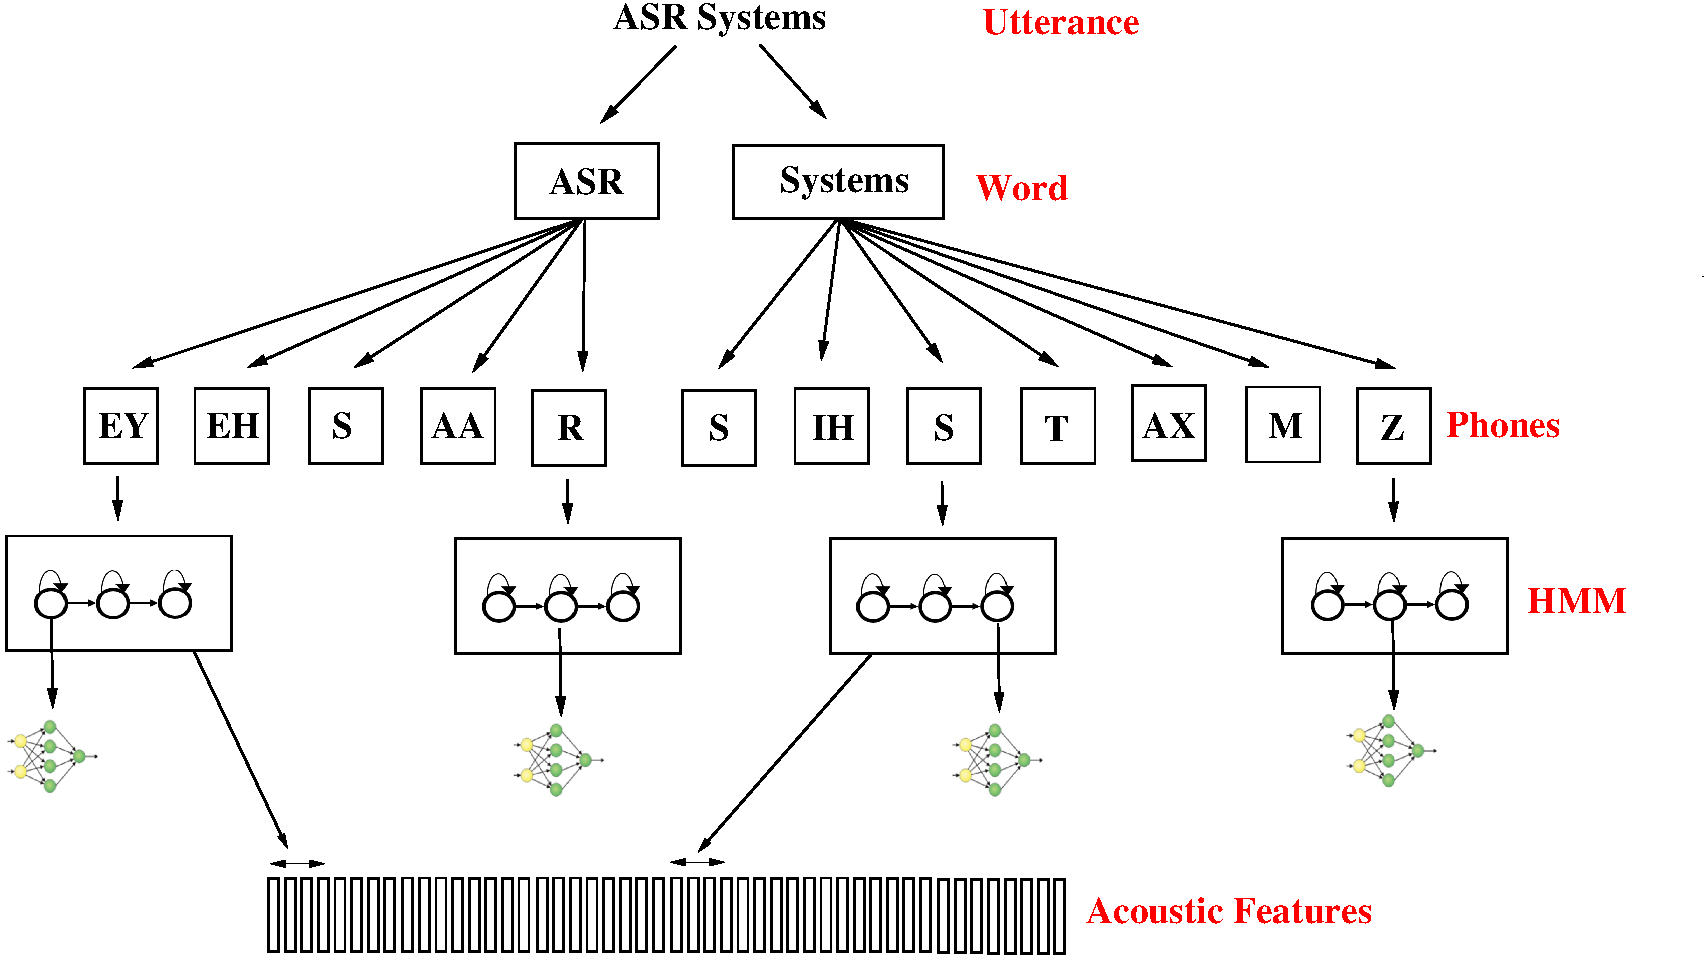
\includegraphics[height=65mm]{figures/am-mlp}
\end{center}
\end{frame}

\begin{frame}{Acoustic Modeling - Current Techniques}
\begin{enumerate}
\item The \alert{basic} model -
\begin{enumerate}
\item Train neural networks to estimate posterior probabilities of speech classes
\item Instead of GMM based likelihood estimates use scaled likelihoods based
off neural network posterior probabilities
\item Trained to discriminate between output classes with a cross-entropy
based training criteria.
\end{enumerate}
\item \alert{Improvements to the basic model} -
\begin{enumerate}
\item Deeper networks, output states corresponding to context dependent states, 
\item Various configurations - CNNs, RNNs, LSTMs
\item Modeling using larger context and correlated features
\item Tigher integration of feature extraction and acoustic modeling
\end{enumerate}
\end{enumerate}
\end{frame}

\begin{frame}{What's under the hood for ASR?}
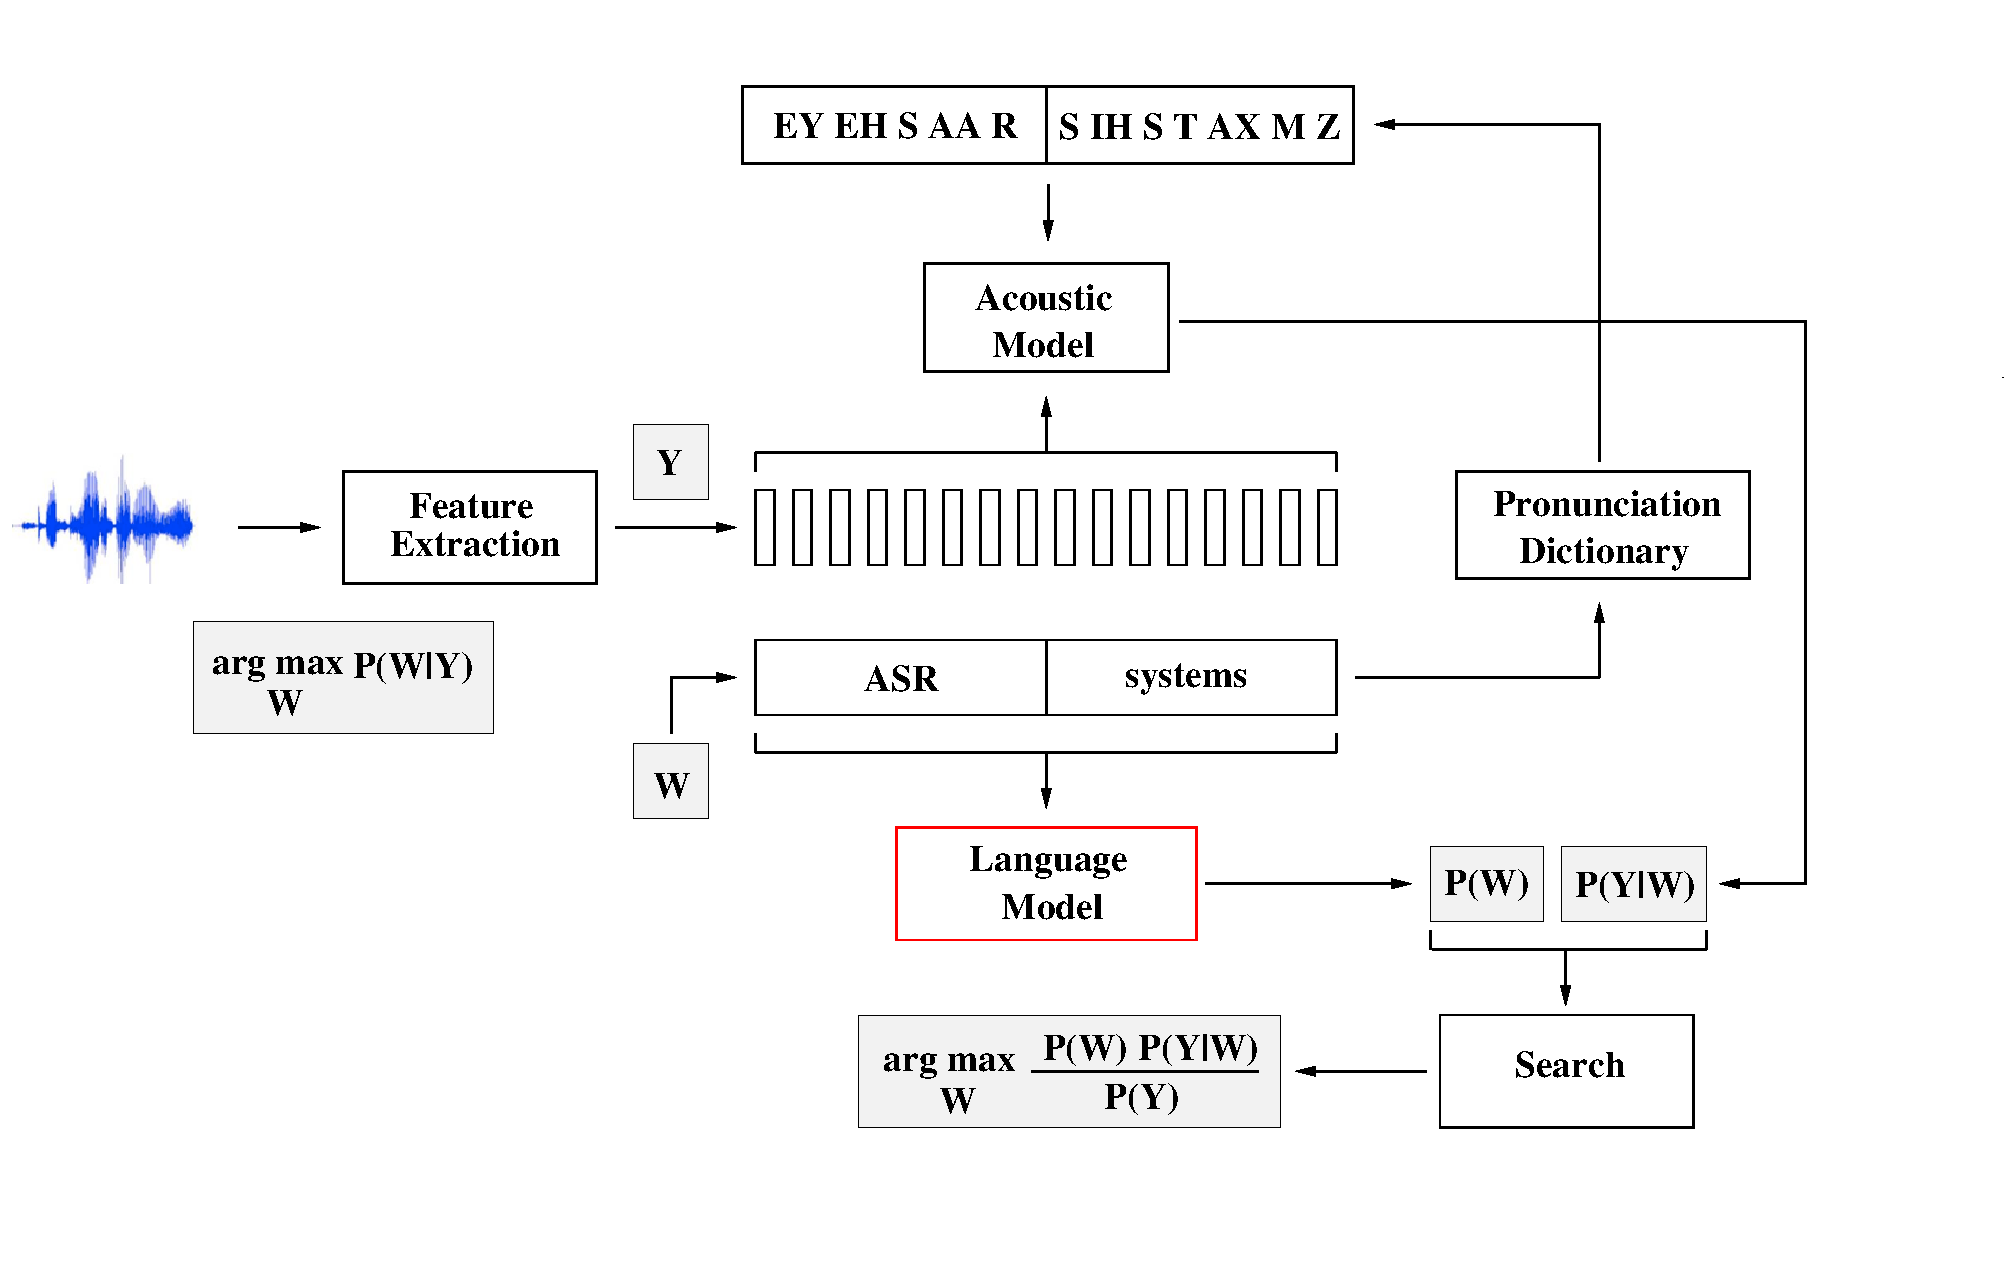
\includegraphics[height=77mm]{figures/b3}
\end{frame}

\begin{frame}{Language Modeling - Introduction}
\begin{enumerate}
\item Estimate the \alert{prior probability} of a word sequence $P(W)$
\item Provides the ASR system with \alert{information about contextual relationships} at a much higher word level
\item Helps \alert{constrain the search space} by helping disambiguate between word sequences that 
sound acoustically similar - "recognize speech" vs. "wreck a nice beach"
\end{enumerate}
\end{frame}

\begin{frame}{Language Modeling - "Past" Techniques}
%Ngrams
%Class based models
\begin{enumerate}
\item The \alert{basic} model -
	\begin{enumerate}
	\item Simple \alert{n-grams} based language models
	\item Probability of a word depends on the word and preceding n-1 words
	\item For a word sequence $W$ = $w_1,w_2,\dots,w_N$, \\
        \begin{center}$P(W)$ = $P(w_1)P(w_2|w_1)P(w_3|w_1,w_2)\dots P(w_N|w_1,w_2,\dots w_{N-1})$\end{center}
	\item A bigram approximation limits the context to one word \\
        \begin{center}$P(W)$ $\simeq$ $P(w_1)P(w_2|w_1)P(w_3|w_2)\dots P(w_N|w_{N-1})$\end{center}
        \item Maximum likelihood estimates for conditional probabilities using counts\\
        \begin{center}$P(w_i|w_j)$ = $\frac{c(w_j,w_i)}{c(w_j)}$\end{center}
	\item Unseen ngrams accounted for using smoothing/discounting/backoff
	\end{enumerate}
\item \alert{Improvements to the basic model} -
	\begin{enumerate}
	\item Class-based n-grams, maximum entropy language models
	\end{enumerate}
\end{enumerate}
\end{frame}

\begin{frame}{Language Modeling - Current Techniques}
\begin{center}
Neural network based language models \\

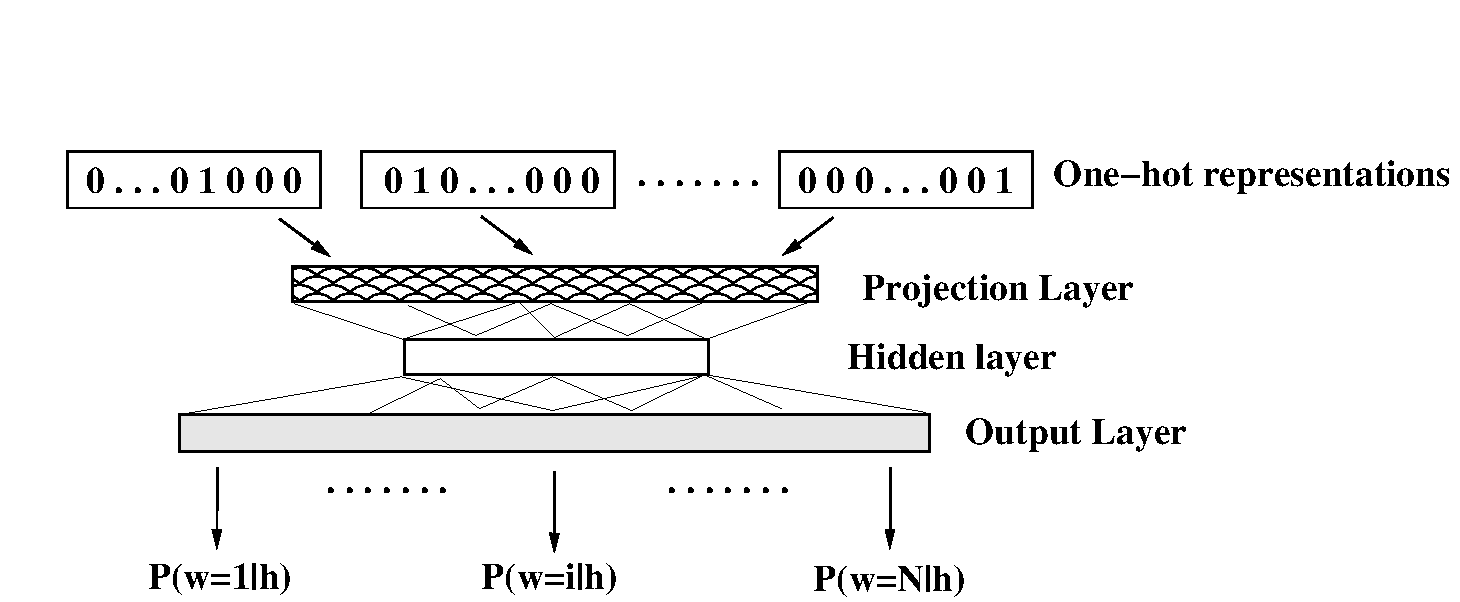
\includegraphics[height=40mm]{figures/lm-mlp}
\end{center}
\end{frame}

\begin{frame}{What's under the hood for ASR?}
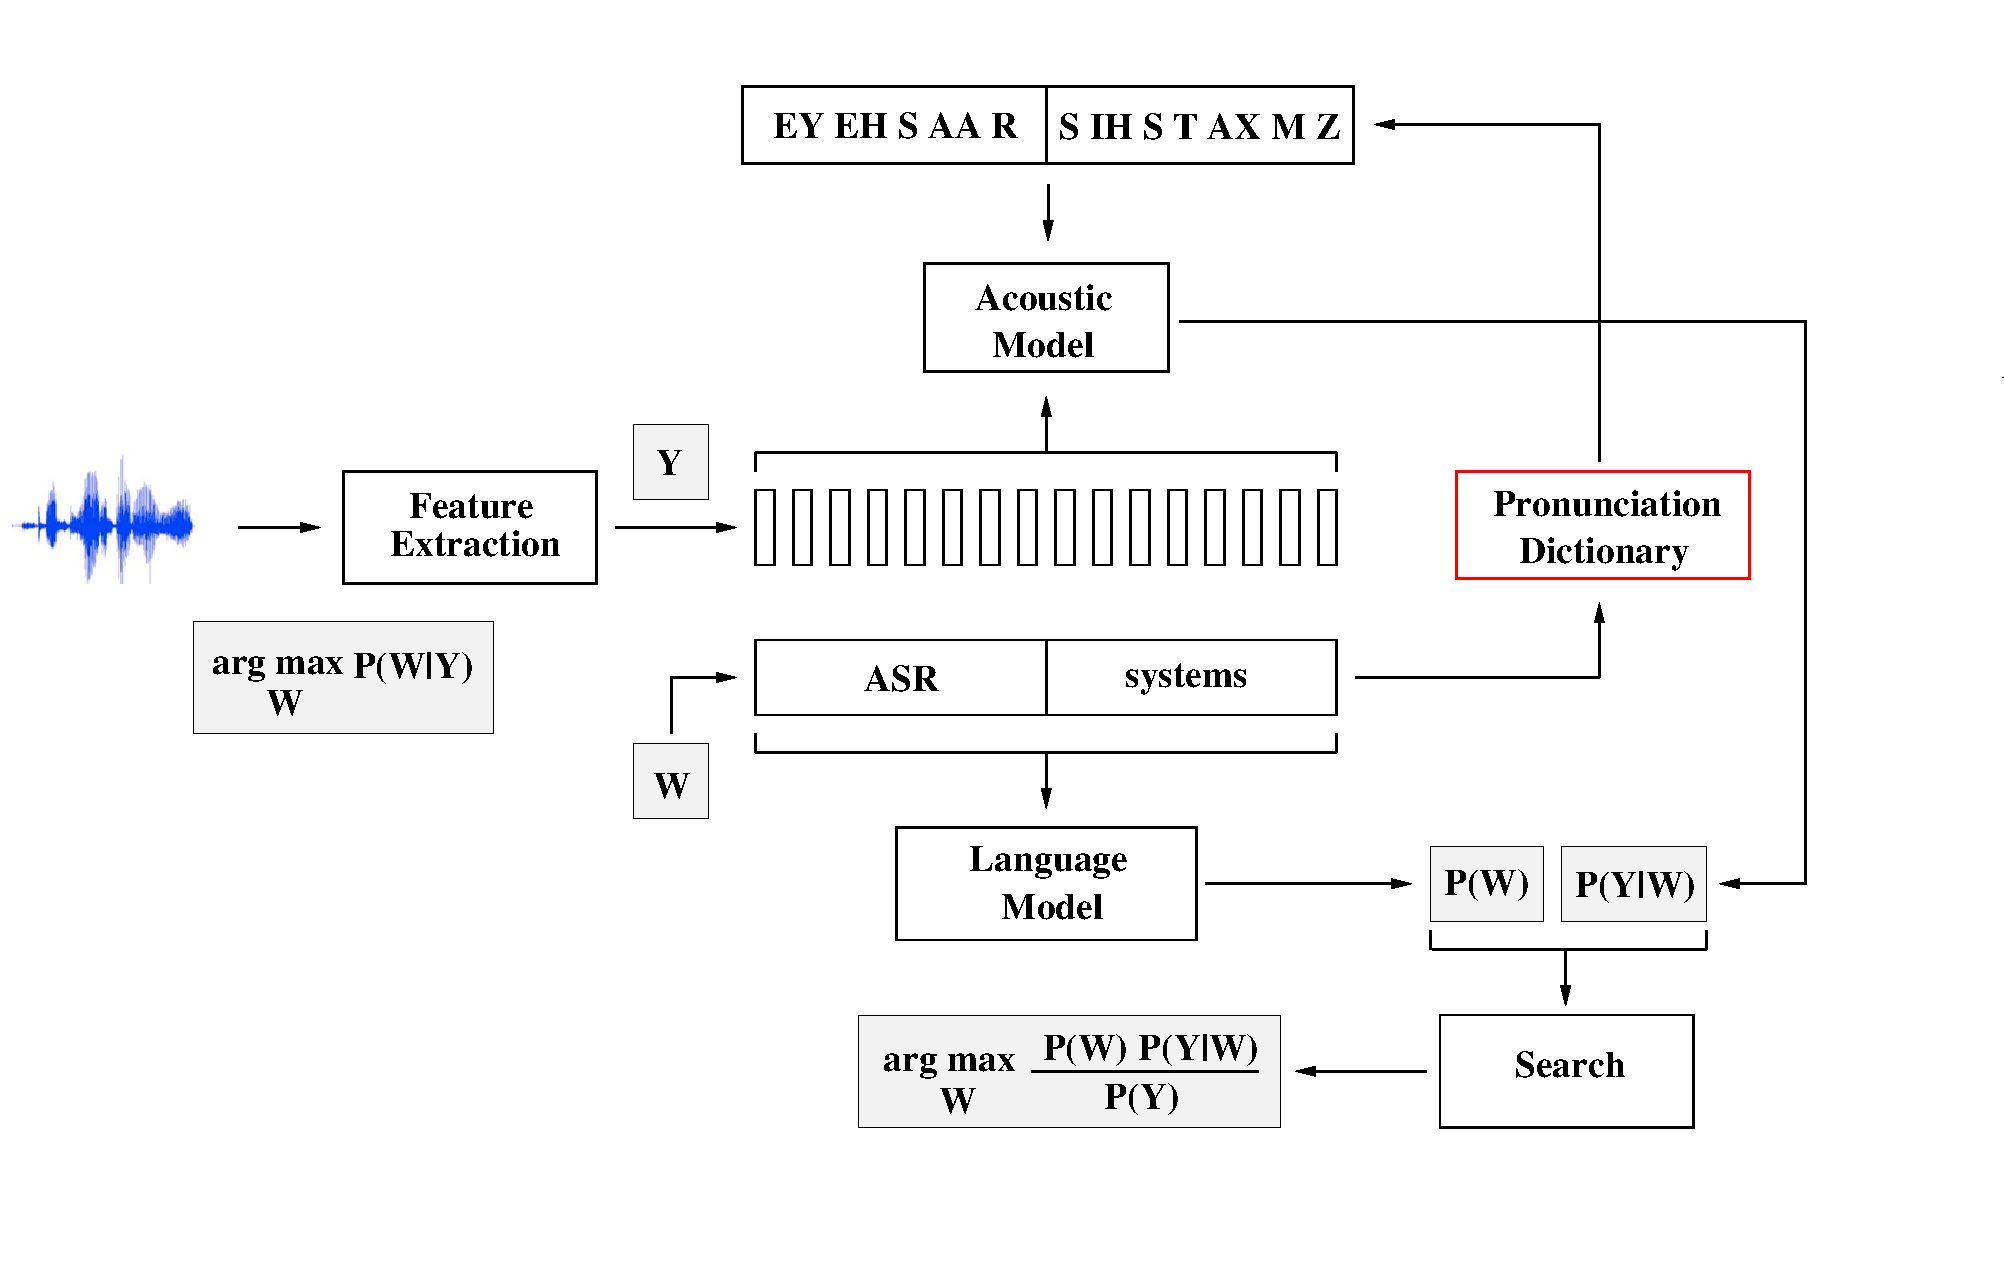
\includegraphics[height=77mm]{figures/b4}
\end{frame}

\begin{frame}{Pronunciation Lexicon}
\begin{enumerate}
\item Provides pronunciations of words \alert{linking} the AM and LM
\item Typically words are represented \alert{phonetically}
\begin{center}
vases(01)                      V EY Z IH Z \\
\end{center}
\item Pronunciation \alert{variants} also need to be added\\
\begin{center}
vases(01)                      V EY Z IH Z \\
vases(02)                      V AA Z IH Z \\
vases(03)                      V EY S IH Z \\
\end{center}
\item \alert{Expensive} since pronunciations are created by human experts
\end{enumerate}
\end{frame}

\begin{frame}{Pronunciation Lexicon}
\begin{enumerate}
\item The \alert{basic} model -
\begin{enumerate}
\item Dictionary created by human experts
\item Grapheme-to-phoneme models - learn pronunciations of words based on initial dictionary
\end{enumerate}
\item \alert{Morphologically rich languages} - modeling at morph level
\begin{enumerate}
\item Compounding (eg. German)
\item Highly inflected languages (eg. Slavic languages)
\item Inflection and compounding (eg. Finnish)
\end{enumerate}
\item \alert{Graphemic dictionaries} - modeling at the character level - bypass the need for pronunciations
\end{enumerate}
\end{frame}

\begin{frame}{What's under the hood for ASR?}
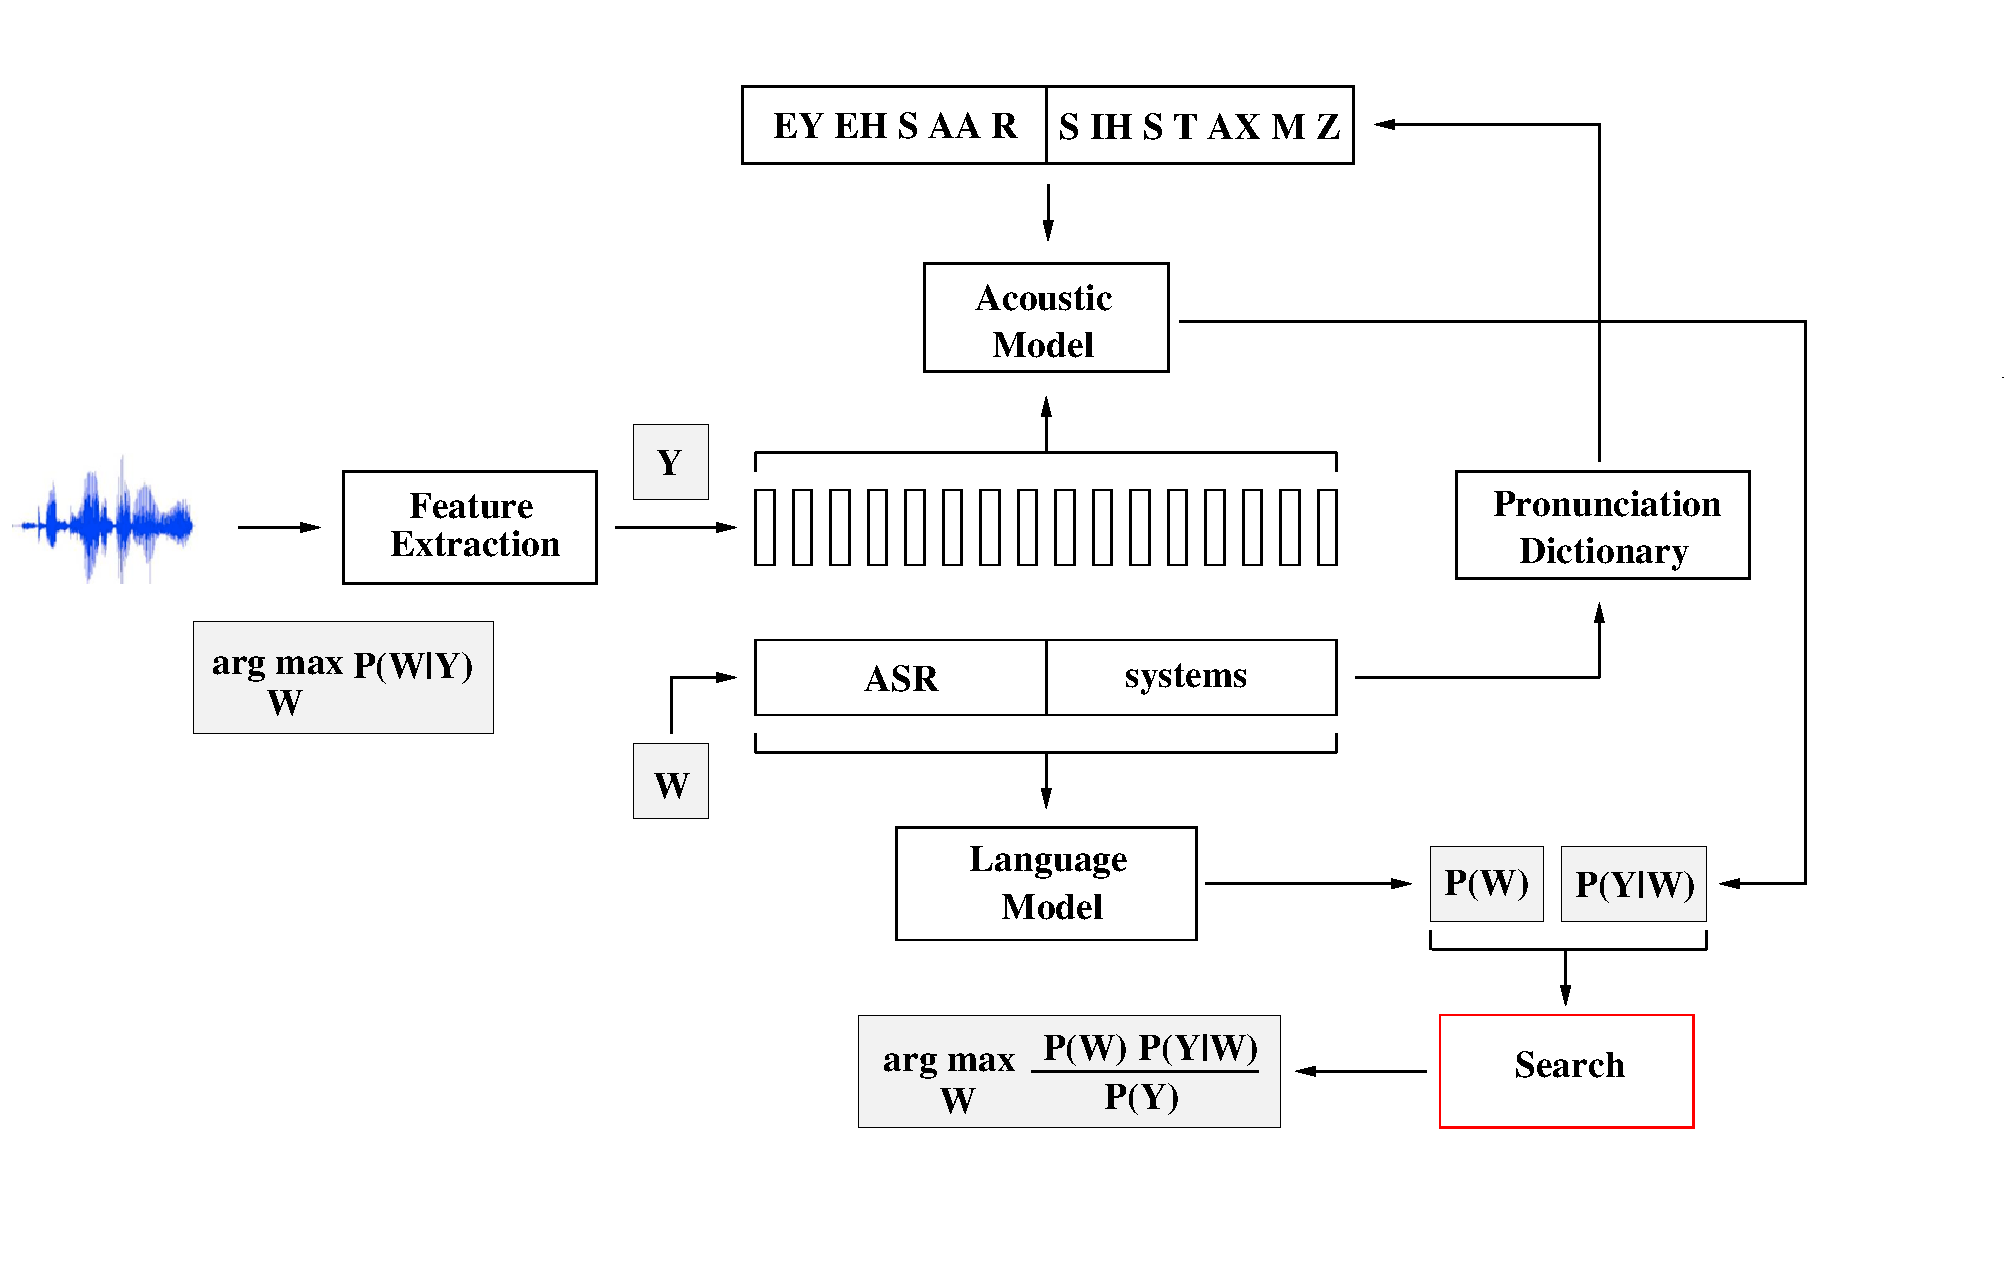
\includegraphics[height=77mm]{figures/b5}
\end{frame}

\begin{frame}{The Decoder}
\begin{enumerate}
\item HMM-based speech recognition - \alert{Viterbi decoding} - efficient dynamic programming based 
search for optimal exhaustive search
\item Search for large vocabulary task is \alert{complex} -
\begin{enumerate}
\item Cross-word triphones and word boundaries
\item Huge search spaces with long-span language models
\end{enumerate}
\item Improved techniques for search -
\begin{enumerate}
\item Beam pruning
\item Multipass search
\item Dynamic networks
\item Weighted finite state transducers
\end{enumerate}
\end{enumerate}
\end{frame}

\begin{frame}{New Languages and Domains - More specifics!}
\begin{columns}[T]
\column{2in}
\centering
{\color{orange}{New Languages}}
\begin{enumerate}
\item Every language is \alert{unique} although they might share many constructs with other languages
\item \alert{Separate resources} specific to the language for building ASR systems are required
\begin{enumerate}
\item Feature extraction
\item Acoustic models
\item Language models
\item Pronunciation lexicons
\end{enumerate}
\item \alert{Building a new ASR system from scratch}
\end{enumerate}
\column{2in}
\centering
{\color{ForestGreen}{New Domains}}
\begin{enumerate}
\item Domains might have specific constructs but usually involves \alert{tailoring existing resources} of a language
\item Resources from the same languages can be \alert{shared}
\begin{enumerate}
\item Feature extraction
\item Acoustic models
\item Language models
\item Pronunciation lexicons
\end{enumerate}
\item Usually \alert{an ASR adaptation problem} rather than building from scratch
\end{enumerate}
\end{columns}
\end{frame}
